\documentclass[BTech]{audiss}
\usepackage{times}
\usepackage{t1enc}
\usepackage{url}
\usepackage{color}
\usepackage{graphicx}
\usepackage{pdfpages}
\usepackage{ifpdf}
\ifpdf
\usepackage[colorlinks=,linkcolor=blue,urlcolor=blue,citecolor=blue,plainpages=false,pdfpagelabels,breaklinks]{hyperref}
\else
\usepackage[colorlinks,linkcolor=blue,urlcolor=blue,citecolor=blue,plainpages=false,pdfpagelabels,linktocpage]{hyperref}
\fi
\usepackage{epstopdf}
\usepackage{amsmath,amssymb}
\usepackage{array}
\usepackage{listings}
\usepackage{xcolor}
\usepackage{ragged2e}
\usepackage{microtype}
\usepackage{booktabs}
\usepackage{multirow}
\usepackage{float}
\usepackage{subcaption}
\sloppy

\usepackage{titlesec}

\titleformat{\chapter}[display]
  {\fontsize{14}{16}\selectfont\bfseries\centering}
  {\MakeUppercase{\chaptertitlename}\ \thechapter}
  {20pt}
  {\fontsize{14}{16}\selectfont\bfseries\MakeUppercase}

\titleformat{name=\chapter,numberless}[display]
  {\fontsize{14}{16}\selectfont\bfseries\centering}
  {}
  {0pt}
  {\fontsize{14}{16}\selectfont\bfseries\MakeUppercase}

\titleformat{\section}
  {\fontsize{12}{14.4}\selectfont\bfseries}
  {\thesection}
  {1em}
  {}

\titleformat{\subsection}
  {\fontsize{12}{14.4}\selectfont\bfseries}
  {\thesubsection}
  {1em}
  {}

\titleformat{\subsubsection}
  {\fontsize{12}{14.4}\selectfont\bfseries}
  {\thesubsubsection}
  {1em}
  {}

\titlespacing*{\chapter}{0pt}{0pt}{20pt}
\titlespacing*{\section}{0pt}{12pt}{6pt}
\titlespacing*{\subsection}{0pt}{12pt}{6pt}
\titlespacing*{\subsubsection}{0pt}{12pt}{6pt}

\lstset{
    basicstyle=\ttfamily\small,
    breaklines=true,
    frame=single,
    keywordstyle=\color{blue},
    stringstyle=\color{teal},
    commentstyle=\color{gray},
}

\begin{document}

% =====================================================================
% TITLE PAGE
% =====================================================================
\begin{titlepage}
\centering
\vspace*{0.5cm}

{\bfseries\large MAJOR PROJECT REPORT\\[0.6em]}
{\normalfont\large On\\[0.8em]}
{\LARGE\textbf{\textit{``Smart Waste Segregation System Using Deep Learning''}}}\\[1.5em]

{\small Submitted in partial fulfilment of the requirements for the award of\\[0.6em]
\textbf{Master of Computer Applications (MCA)\\[0.6em]
In the department of\\[0.6em]
\textbf{Computer Applications}}\\[2em]

\vspace{0.5cm}

\includegraphics[width=0.35\textwidth]{au.jpg}\\[1.5em]

{\itshape Submitted by:}\\[0.6em]
{\bfseries Minarul Hoque (PG/SOET/28/24/060)}\\[0.4em]
{\bfseries Rohan Dey (PG/SOET/28/24/062)}\\[0.4em]
{\bfseries Ritwik Ghosh (PG/SOET/28/24/004)}\\[0.4em]
{\bfseries Raktim Kumar (PG/SOET/28/24/005)}\\[0.4em]
{\bfseries Ataur Rahaman Din (PG/SOET/28/24/043)}\\[2.5em]

{\itshape Under the Guidance of}\\[0.6em]
{\bfseries Dr. Debdutta Pal}\\
{(Associate Professor)}\\[1em]

\vfill
{\small \textbf{School of Engineering \& Technology}\\
\textbf{ADAMAS University, Kolkata, West Bengal}\\
JAN 2026 -- JUN 2026}}

\end{titlepage}

% =====================================================================
% CERTIFICATE
% =====================================================================
\pagenumbering{roman}
\setcounter{page}{1}

\addcontentsline{toc}{chapter}{CERTIFICATE}
\begin{center}
{\Large \textbf{CERTIFICATE}}\\[1.5em]
\end{center}

\vspace{1em}
\noindent
This is to certify that the project report entitled \textit{``Smart Waste Segregation System Using Deep Learning''}, submitted to the School of Engineering \& Technology (SOET), \textbf{ADAMAS UNIVERSITY, KOLKATA} in partial fulfilment for the completion of the degree of \textbf{Master of Computer Applications} in the department of \textbf{Computer Applications}, is a record of bonafide work carried out by \textbf{Minarul Hoque (PG/SOET/28/24/060), Rohan Dey (PG/SOET/28/24/062), Ritwik Ghosh (PG/SOET/28/24/004), Raktim Kumar (PG/SOET/28/24/005), Ataur Rahaman Din (PG/SOET/28/24/043)} under our guidance.\\[1em]
All help received from various sources has been duly acknowledged.\\
No part of this report has been submitted elsewhere for the award of any other degree.\\[4em]

\begin{center}
\rule{8cm}{0.4pt}\\
{\textbf{Dr. Debdutta Pal}}\\
{(Associate Professor, Department of Computer Applications)}\\[3em]

\rule{8cm}{0.4pt}\\
{\textbf{Mr. Aninda Kundu / Mr. Sayantan Singha Roy}}\\
{(Project Coordinator)}\\[3em]

\rule{8cm}{0.4pt}\\
{\textbf{Dr. Debasish Chakraborty}}\\
{(HOD, Department of Computer Applications)}\\[2em]
\end{center}

\pagebreak

% =====================================================================
% ACKNOWLEDGEMENT
% =====================================================================
\addcontentsline{toc}{chapter}{ACKNOWLEDGEMENT}
\begin{center}
{\Large \textbf{ACKNOWLEDGEMENT}}\\[2em]
\end{center}

We, as the project team, sincerely thank our guide, \textbf{Dr. Debdutta Pal}, Associate Professor, Department of Computer Applications, Adamas University, for his continuous support, expert advice, and constructive suggestions throughout the development of this project. His invaluable guidance helped us navigate complex technical challenges and produce a rigorous, high-quality research outcome.

We express our sincere gratitude to \textbf{Dr. Debasish Chakraborty}, Head of the Department of Computer Applications, for providing an excellent academic environment and the necessary resources to conduct this project successfully.

We are thankful to the \textbf{School of Engineering \& Technology, Adamas University} for granting us access to the NVIDIA L40S GPU infrastructure, which made our deep learning experiments feasible.

We also acknowledge \textbf{Roboflow} for providing the annotation and augmentation platform used in building our dataset, and \textbf{Ultralytics} for the open-source YOLO11 framework that served as the foundation of our work.

Finally, we thank our families and fellow students for their constant encouragement and support throughout this journey.

\pagebreak

% =====================================================================
% DECLARATION
% =====================================================================
\addcontentsline{toc}{chapter}{DECLARATION}
\begin{center}
{\Large \textbf{DECLARATION}}\\[2em]
\end{center}

\noindent
We, the undersigned, declare that the project entitled \textit{``Smart Waste Segregation System Using Deep Learning''}, being submitted in partial fulfillment for the award of Master of Computer Applications, affiliated to ADAMAS University, is the work carried out by us. This project has not been submitted elsewhere for the award of any degree or diploma.\\[6em]

\begin{center}
\begin{tabular}{p{7cm} p{7cm}}
\centering \rule{6cm}{0.4pt} \\[-0.3em]
\centering \textbf{Minarul Hoque} \\ (PG/SOET/28/24/060) \\[2em]
\centering \rule{6cm}{0.4pt} \\[-0.3em]
\centering \textbf{Rohan Dey} \\ (PG/SOET/28/24/062) \\[2em]
\centering \rule{6cm}{0.4pt} \\[-0.3em]
\centering \textbf{Ritwik Ghosh} \\ (PG/SOET/28/24/004) \\[2em]
\centering \rule{6cm}{0.4pt} \\[-0.3em]
\centering \textbf{Raktim Kumar} \\ (PG/SOET/28/24/005) \\[2em]
\centering \rule{6cm}{0.4pt} \\[-0.3em]
\centering \textbf{Ataur Rahaman Din} \\ (PG/SOET/28/24/043) \\[2em]
\end{tabular}
\end{center}

\pagebreak

% =====================================================================
% ABSTRACT
% =====================================================================
\abstract
\vspace*{24pt}

\noindent
The global solid waste management crisis is worsening rapidly, with over 2.01 billion tonnes of municipal solid waste generated annually, yet source-level segregation remains critically low in most developing regions. Manual waste sorting is error-prone, inconsistent, and economically unsustainable. This project presents a \textbf{Smart Waste Segregation System} that automates the classification of waste into \textbf{Biodegradable (Bio)} and \textbf{Non-Biodegradable (Non-Bio)} categories using state-of-the-art deep learning object detection.

The system is built upon an enhanced \textbf{YOLO11s} architecture augmented with a \textbf{Bidirectional Feature Pyramid Network (BiFPN)} neck for improved multi-scale feature fusion and a \textbf{Wise-IoU (WIoU)} loss function for geometrically robust bounding box regression. A \textbf{custom dataset of 3,000 real-world images} was independently collected and manually annotated by the project team using the Roboflow platform, then expanded to \textbf{10,175 images} through systematic augmentation --- forming the publicly released \textbf{WasteManagement-2} benchmark.

Through a rigorous \textbf{eight-step ablation study}, we demonstrate that data augmentation contributes the largest single performance gain (+15.0\% mAP@0.5), while BiFPN provides meaningful multi-scale feature improvement. The final model achieves \textbf{94.39\% mAP@0.5} on the validation set and \textbf{85.46\% mAP@0.5} on the independent held-out test set, at an inference speed of \textbf{4.0\,ms per image}. A fully functional laptop-deployable demo application is provided for real-time waste detection via image upload or webcam.

\noindent KEYWORDS: \hspace*{0.5em} \parbox[t]{4.4in}{Waste Classification, YOLO11, BiFPN, WIoU Loss, Object Detection, Deep Learning, Waste Segregation, Data Augmentation, Ablation Study, Real-Time Detection.}

\pagebreak

% =====================================================================
% TABLE OF CONTENTS
% =====================================================================
\begin{singlespace}
\tableofcontents
\thispagestyle{empty}
\end{singlespace}
\listoftables
\addcontentsline{toc}{chapter}{LIST OF TABLES}
\listoffigures
\addcontentsline{toc}{chapter}{LIST OF FIGURES}

% =====================================================================
% ABBREVIATIONS
% =====================================================================
\abbreviations
\noindent
\begin{tabbing}
xxxxxxxxxxxx \= xxxxxxxxxxxxxxxxxxxxxxxxxxxxxxxxxxxxxxxxxxxxxxxx \kill
\textbf{AI}      \> Artificial Intelligence \\
\textbf{API}     \> Application Programming Interface \\
\textbf{AP}      \> Average Precision \\
\textbf{BiFPN}   \> Bidirectional Feature Pyramid Network \\
\textbf{CBAM}    \> Convolutional Block Attention Module \\
\textbf{CNN}     \> Convolutional Neural Network \\
\textbf{COCO}    \> Common Objects in Context \\
\textbf{CPU}     \> Central Processing Unit \\
\textbf{CUDA}    \> Compute Unified Device Architecture \\
\textbf{CV}      \> Computer Vision \\
\textbf{DL}      \> Deep Learning \\
\textbf{FN}      \> False Negatives \\
\textbf{FP}      \> False Positives \\
\textbf{FPN}     \> Feature Pyramid Network \\
\textbf{GFLOPs}  \> Giga Floating Point Operations Per Second \\
\textbf{GPU}     \> Graphics Processing Unit \\
\textbf{HOD}     \> Head of Department \\
\textbf{HSV}     \> Hue, Saturation, Value (colour space) \\
\textbf{IoU}     \> Intersection over Union \\
\textbf{LR}      \> Learning Rate \\
\textbf{mAP}     \> mean Average Precision \\
\textbf{MCA}     \> Master of Computer Applications \\
\textbf{ML}      \> Machine Learning \\
\textbf{MSW}     \> Municipal Solid Waste \\
\textbf{NMS}     \> Non-Maximum Suppression \\
\textbf{ONNX}    \> Open Neural Network Exchange \\
\textbf{P}       \> Precision \\
\textbf{R}       \> Recall \\
\textbf{RGB}     \> Red Green Blue \\
\textbf{SOET}    \> School of Engineering and Technology \\
\textbf{SSD}     \> Single Shot MultiBox Detector \\
\textbf{TN}      \> True Negatives \\
\textbf{TP}      \> True Positives \\
\textbf{VRAM}    \> Video Random Access Memory \\
\textbf{WIoU}    \> Wise Intersection over Union \\
\textbf{YOLO}    \> You Only Look Once \\
\end{tabbing}

\pagebreak

% =====================================================================
% NOTATION
% =====================================================================
\chapter*{\centerline{NOTATION}}
\addcontentsline{toc}{chapter}{NOTATION}

\begin{singlespace}
\begin{tabbing}
xxxxxxxxxxxx \= xxxxxxxxxxxxxxxxxxxxxxxxxxxxxxxxxxxxxxxxxxxxxxxx \kill
\textbf{$P$}              \> Precision: $TP / (TP + FP)$ \\
\textbf{$R$}              \> Recall: $TP / (TP + FN)$ \\
\textbf{$F_1$}            \> F1-Score: $2PR / (P + R)$ \\
\textbf{$\text{AP}$}      \> Area under Precision-Recall curve for one class \\
\textbf{$\text{mAP}$}     \> Mean Average Precision across all classes \\
\textbf{$\text{IoU}$}     \> Intersection over Union between predicted and ground-truth box \\
\textbf{$w_i$}            \> Learnable BiFPN fusion weight for feature level $i$ \\
\textbf{$\varepsilon$}    \> Small constant ($10^{-4}$) for numerical stability \\
\textbf{$\mathcal{O}$}    \> BiFPN output feature map after weighted fusion \\
\textbf{$I_i$}            \> Input feature map at level $i$ \\
\textbf{$\mathcal{L}$}    \> Total training loss function \\
\textbf{$\mathcal{L}_{\text{WIoU}}$} \> Wise-IoU bounding box regression loss \\
\textbf{$r$}              \> WIoU dynamic focusing coefficient \\
\textbf{$lr_0$}           \> Initial learning rate \\
\textbf{$lr_f$}           \> Final learning rate after cosine annealing \\
\textbf{$B$}              \> Batch size \\
\textbf{$E$}              \> Number of training epochs \\
\textbf{$P3, P4, P5$}     \> Feature pyramid levels at strides 8, 16, 32 \\
\textbf{$n$}              \> Number of images in dataset split \\
\textbf{$C$}              \> Number of classes (2: Bio, Non-Bio) \\
\end{tabbing}
\end{singlespace}

\pagebreak
\clearpage
\pagenumbering{arabic}

% =====================================================================
% CHAPTERS
% =====================================================================
\chapter{INTRODUCTION}

\section{Background}

Waste management has emerged as one of the most critical environmental and public health challenges of the modern era. Rapid urbanisation, population growth, and changing consumption patterns have led to an unprecedented increase in the volume and complexity of municipal solid waste (MSW) generated globally. According to the World Bank's \textit{What a Waste 2.0} report \cite{worldbank2018}, approximately \textbf{2.01 billion tonnes} of solid waste is generated worldwide every year, a figure projected to grow to \textbf{3.4 billion tonnes by 2050} if no corrective measures are taken. In developing countries, improper waste disposal is responsible for significant environmental degradation, soil contamination, water pollution, and the spread of infectious diseases.

A fundamental prerequisite for effective waste management is proper waste \textbf{segregation at the point of generation} — the process of separating waste into distinct categories based on its material composition and biodegradability. Biodegradable waste, such as food scraps, plant matter, and organic materials, can be composted or treated through anaerobic digestion to produce biogas and organic fertiliser. Non-biodegradable waste, including plastics, metals, glass, and electronic components, requires separate collection streams for recycling, incineration, or controlled landfilling.

Despite the well-established benefits of source segregation, implementation remains alarmingly poor. Studies report that less than \textbf{5\%} of waste is properly segregated at the household or institutional level in most developing economies \cite{systematic_review2025}. Manual sorting operations in waste processing facilities carry error rates exceeding \textbf{20\%}, are labour-intensive, and expose workers to significant health hazards. These inefficiencies result in large volumes of recyclable and compostable material being directed to landfills, reducing resource recovery and increasing greenhouse gas emissions.

Artificial intelligence, and deep learning in particular, offers a transformative opportunity to automate waste classification with high accuracy, consistency, and speed. Object detection models can identify and localise waste items in images or video streams, enabling automated bin-sorting systems, smart waste collection infrastructure, and real-time monitoring platforms.

\section{Problem Statement}

The core problem this project addresses is as follows:

\textit{Existing manual waste segregation methods are unreliable, slow, and costly. There is a need for an accurate, real-time, automated system capable of classifying waste into Biodegradable and Non-Biodegradable categories from camera input, suitable for practical deployment without specialised hardware.}

Specifically, the challenges include:
\begin{enumerate}
    \item High visual similarity between certain biodegradable and non-biodegradable items (e.g., paper vs. cardboard, food wrappers vs. organic matter).
    \item Variable waste appearance due to partial occlusion, irregular shapes, and co-mingled waste scenarios.
    \item The need for real-time performance — classification must occur within milliseconds for conveyor belt or bin-gate actuation.
    \item Dataset scarcity: publicly available waste datasets are limited in diversity and volume.
    \item Architectural complexity versus accuracy trade-off: adding components to a model does not always improve performance.
\end{enumerate}

\section{Motivation}

The motivation for this project arises from both the scale of the waste crisis and the demonstrated potential of deep learning for visual recognition tasks. The following factors drive the development of this system:

\begin{itemize}
    \item \textbf{Environmental Impact:} Effective waste segregation reduces landfill burden, lowers methane emissions from biodegradable decomposition, and maximises recyclable material recovery.
    \item \textbf{Health and Safety:} Automating waste sorting reduces human exposure to hazardous materials and pathogenic waste.
    \item \textbf{Economic Value:} Properly segregated waste has significant secondary market value through composting and recycling, creating economic incentives for automation.
    \item \textbf{Technological Readiness:} Modern object detection frameworks such as YOLO and architectural innovations like BiFPN have made accurate, real-time visual classification practically achievable on commodity hardware.
    \item \textbf{Research Gap:} Prior work lacks systematic ablation studies that isolate the contribution of individual model components, making principled architectural decisions difficult.
\end{itemize}

\section{Objectives}

The primary objectives of this project are:

\begin{enumerate}
    \item To collect and annotate a custom waste image dataset comprising \textbf{3,000 raw images} covering both biodegradable and non-biodegradable waste categories across diverse environments.
    \item To design and implement a deep learning-based waste classification system using the \textbf{YOLO11s} architecture enhanced with a \textbf{BiFPN neck} and \textbf{WIoU loss function}.
    \item To conduct a \textbf{systematic eight-step ablation study} evaluating the individual and combined contributions of data augmentation, attention mechanisms (CBAM), bidirectional feature fusion (BiFPN), advanced loss functions (WIoU), and deformable convolutions.
    \item To achieve a classification accuracy of at least \textbf{93\% mAP@0.5} on the validation set.
    \item To develop a \textbf{real-time demo application} deployable on a standard laptop for live waste detection via image upload or webcam.
    \item To produce a \textbf{research publication} in Springer LNCS format documenting the methodology and findings.
\end{enumerate}

\section{Scope of the Project}

This project operates within the following scope:

\begin{itemize}
    \item \textbf{Classification scope:} Binary classification — Biodegradable (Bio) and Non-Biodegradable (Non-Bio) waste.
    \item \textbf{Input modality:} RGB images (640$\times$640 pixels) captured by standard cameras, mobile phones, or webcams.
    \item \textbf{Deployment:} Software-only system running on CPU/GPU-equipped laptops or desktops. Physical hardware integration (robotic arms, conveyor belts) is considered future work.
    \item \textbf{Dataset:} Custom dataset of 3,000 images collected and annotated by the project team, augmented to 10,175 training-ready images.
    \item \textbf{Training infrastructure:} NVIDIA L40S GPU (46\,GB VRAM) provided by Adamas University's AI/ML research computing cluster.
    \item \textbf{Framework:} PyTorch and Ultralytics YOLO11.
\end{itemize}

\section{Overview of the Proposed System}

The proposed system consists of four major components:

\begin{enumerate}
    \item \textbf{Dataset Pipeline:} Raw image collection (photography and internet), annotation via Roboflow, augmentation to expand training diversity.
    \item \textbf{Model Architecture:} YOLO11s backbone with BiFPN neck and WIoU-optimised anchor-free detection head.
    \item \textbf{Training and Evaluation:} Systematic eight-step ablation study, with final model trained for 100 epochs using AdamW optimiser with cosine annealing.
    \item \textbf{Demo Application:} Streamlit-based web application supporting image upload and live webcam detection with confidence scores and class labels.
\end{enumerate}

Figure~\ref{fig:architecture} shows the overall architecture of the proposed system.

\begin{figure}[H]
    \centering
    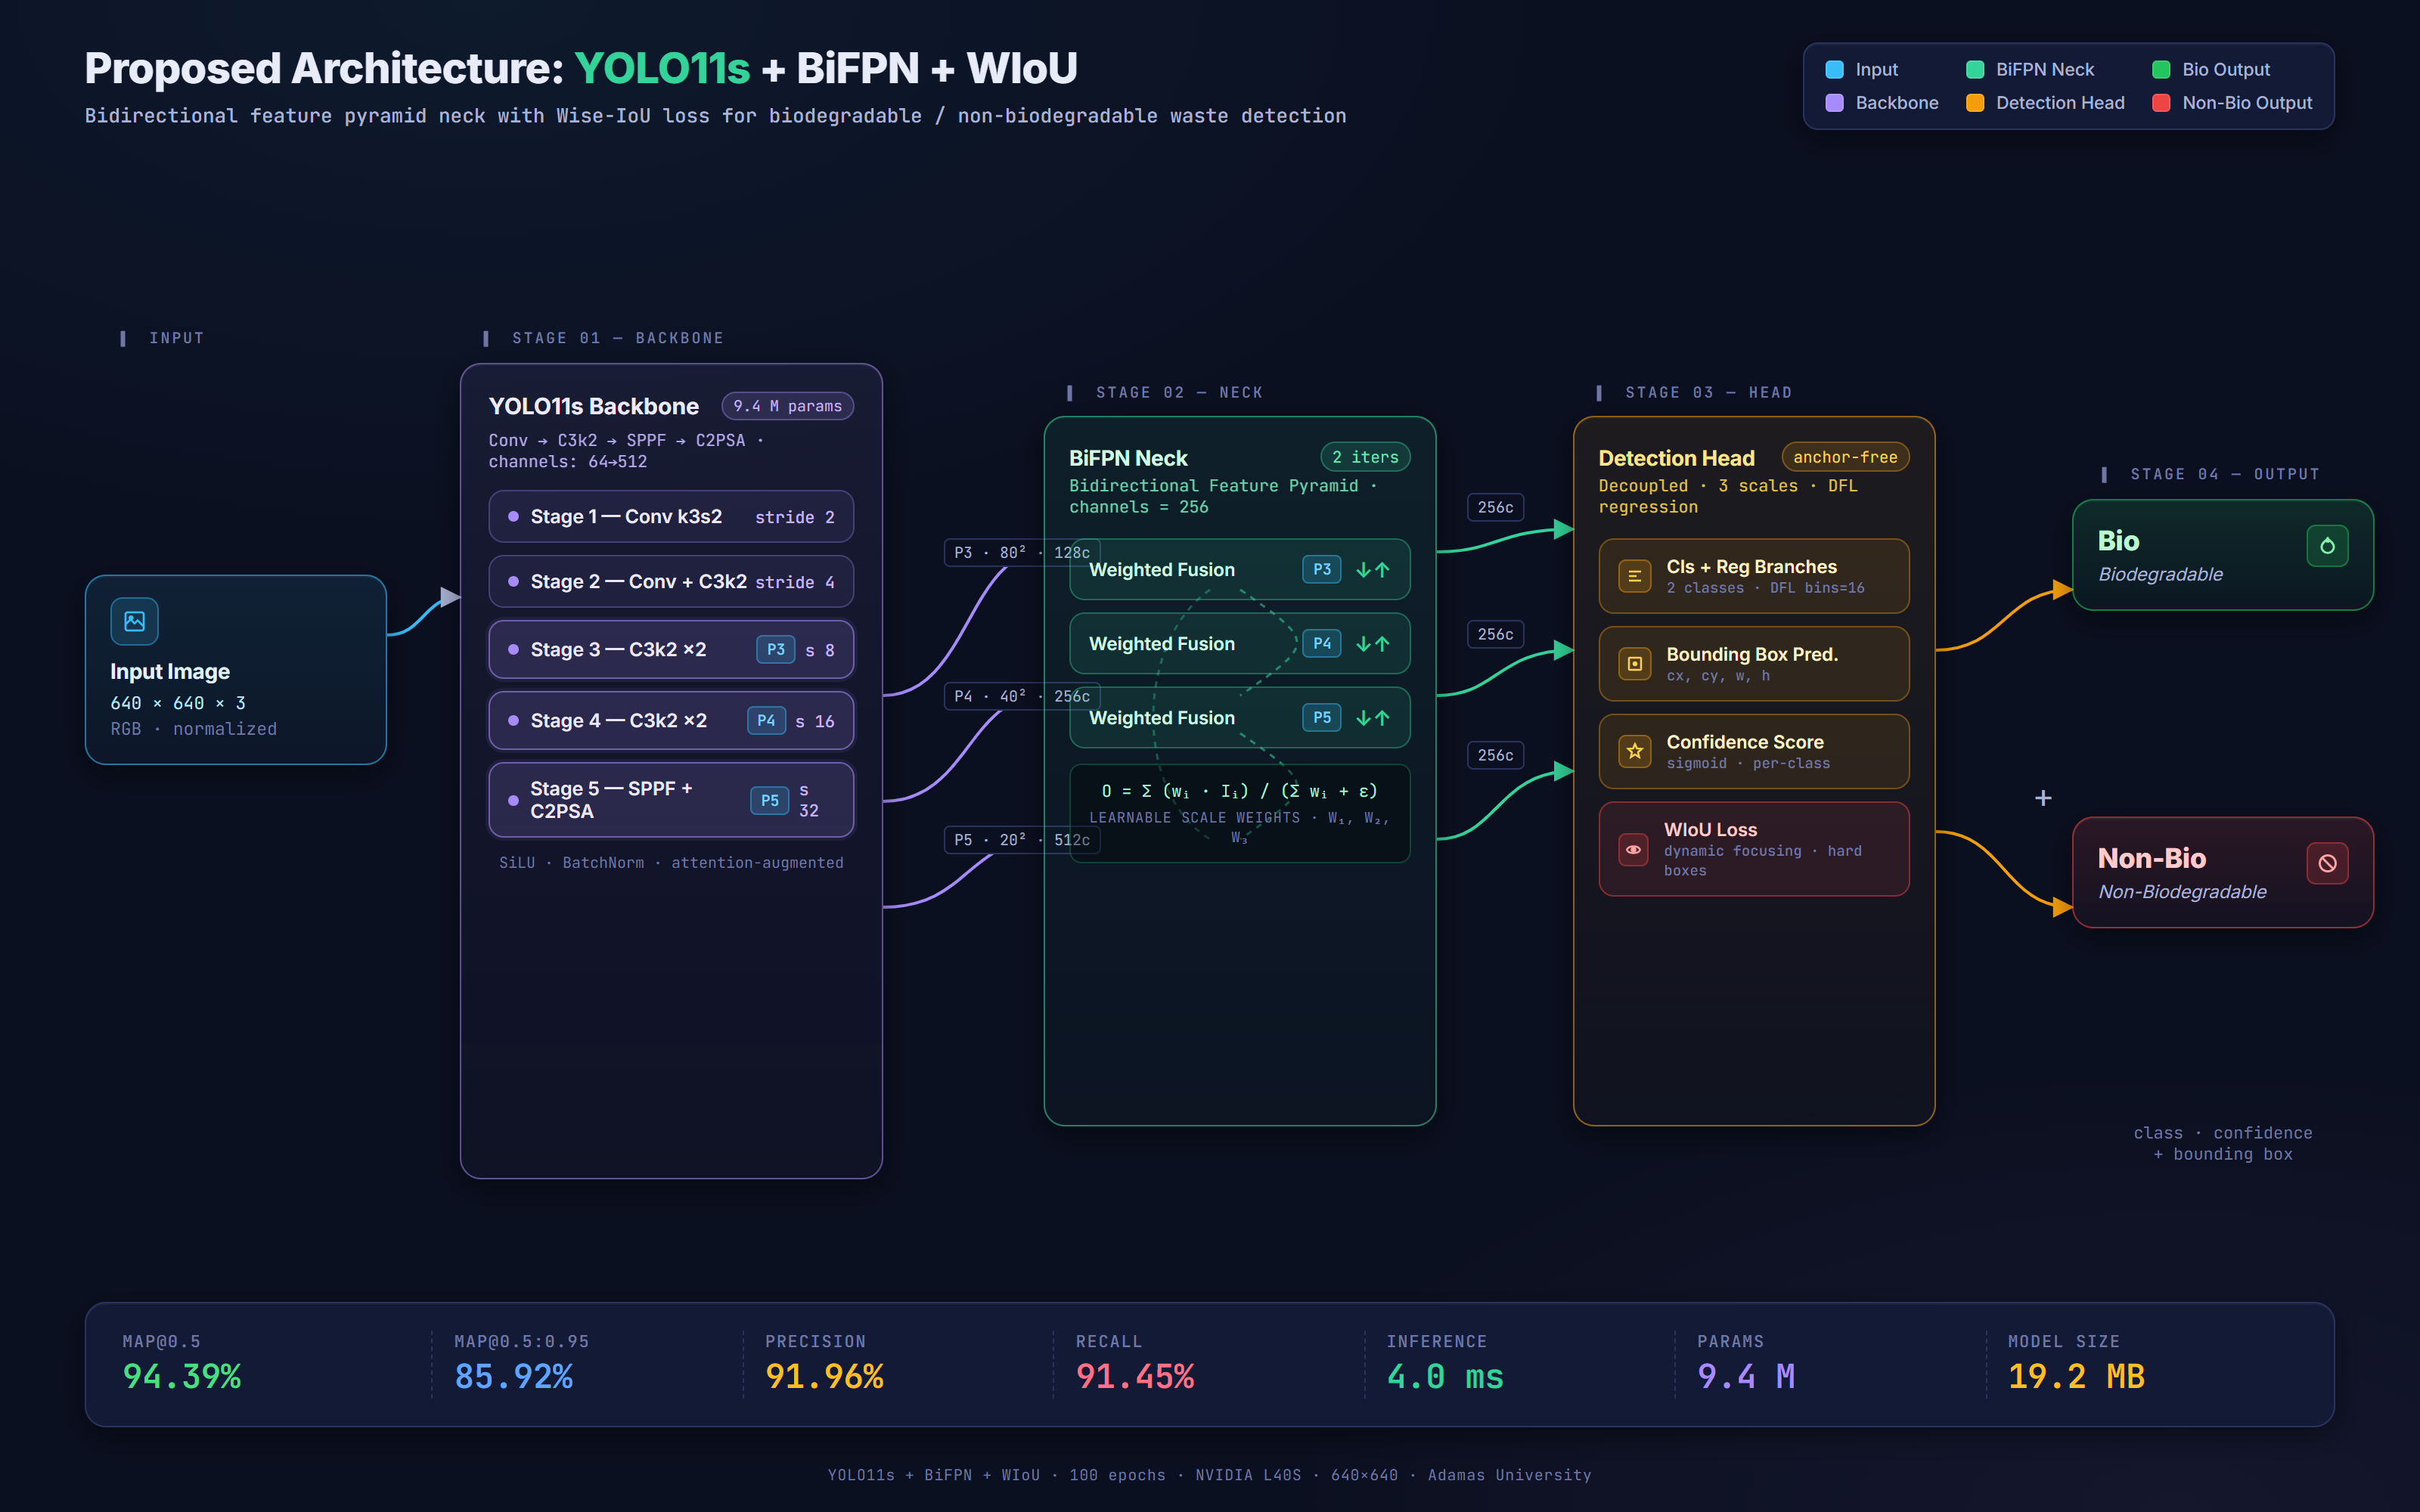
\includegraphics[width=\textwidth]{images/architecture_diagram.png}
    \caption{Proposed System Architecture: YOLO11s + BiFPN + WIoU}
    \label{fig:architecture}
\end{figure}

\section{Key Contributions}

This project makes the following original contributions:

\begin{enumerate}
    \item \textbf{Public Waste Detection Dataset:} A 3,000-image manually annotated dataset covering mixed indoor and outdoor waste scenarios — diverse backgrounds, partial occlusion, fresh and degraded items — expanded to 10,175 images through structured augmentation and released publicly on Roboflow Universe under CC BY 4.0.
    \item \textbf{Systematic Ablation Study:} An eight-step controlled experiment isolating the contribution of each architectural component — the first such study of this scope for binary waste detection, directly addressing a gap identified by recent systematic reviews.
    \item \textbf{Evidence-Based Architecture:} Empirical demonstration that data augmentation (+15.0\% mAP@0.5) dominates all architectural changes combined, and that WIoU v3 with BiFPN provides the best accuracy-complexity trade-off, while CBAM and deformable convolutions degrade performance on this task.
    \item \textbf{High-Performance Model:} Final YOLO11s + BiFPN + WIoU v3 model achieving \textbf{94.39\% mAP@0.5} on the validation set and \textbf{85.46\% mAP@0.5} on the independent held-out test set, at 4.0\,ms GPU inference latency with a 19.2\,MB model footprint.
    \item \textbf{Deployable Demo Application:} A fully functional real-time Streamlit application supporting image upload and webcam detection — addressing the widely noted absence of deployment-ready open systems in the waste classification research community.
\end{enumerate}

\section{Organisation of the Report}

The remainder of this report is organised as follows:

\begin{itemize}
    \item \textbf{Chapter 2 — Literature Review:} Reviews ten existing works in waste classification, IoT-based systems, and YOLO-based detection. Identifies research gaps addressed by this project.
    \item \textbf{Chapter 3 — Technology:} Describes all software frameworks, libraries, and hardware used in this project.
    \item \textbf{Chapter 4 — System Design:} Presents functional and non-functional requirements, system architecture, data flow, and module descriptions.
    \item \textbf{Chapter 5 — Methodology:} Details the dataset construction process, model architecture design decisions, training strategy, and evaluation metrics.
    \item \textbf{Chapter 6 — Implementation:} Describes the practical implementation of each component, including dataset preparation, training code, ablation experiments, and the demo application.
    \item \textbf{Chapter 7 — Results and Analysis:} Presents and analyses all experimental results including the ablation study, final model performance, per-class metrics, and visual outputs.
    \item \textbf{Chapter 8 — Conclusion:} Summarises the project's achievements and key findings.
    \item \textbf{Chapter 9 — Future Work:} Proposes directions for extending this work.
\end{itemize}

\chapter{LITERATURE REVIEW}

\section{Introduction}

This chapter reviews existing literature on automated waste classification, object detection architectures, and smart waste management systems. The review covers eight significant works that have shaped the research landscape and identifies the specific gaps this project addresses. The papers are organised by thematic area: early deep learning approaches, hardware-integrated classification systems, YOLO-based detection methods, feature pyramid enhancements, and systematic reviews.

\section{Review of Existing Works}

\subsection{Auto Classification of Biodegradable and Non-Biodegradable Objects (2017)}

One of the earliest works addressing binary waste classification using machine vision \cite{autoclassify2017} established the foundational framework for automated biodegradable versus non-biodegradable segregation. The authors employed a CNN-based classifier trained on a relatively small dataset of controlled laboratory images. While the system demonstrated proof-of-concept viability, it was limited by: (i) low dataset diversity with single-item images under controlled lighting, (ii) static background conditions that would not generalise to real-world cluttered environments, and (iii) a classification-only approach without spatial localisation of waste items. This work remains a key reference as it defined the binary classification problem that subsequent works, including this project, seek to solve at higher accuracy and real-world applicability.

\subsection{Deep Learning Based Waste Segregation Using SSD and MobileNet (2021)}

This work \cite{ssd_mobilenet2021} deployed a Single Shot MultiBox Detector (SSD) combined with a MobileNet backbone on a Raspberry Pi for real-time embedded waste detection. The lightweight MobileNet backbone was chosen to meet the computational constraints of the Raspberry Pi platform. The system demonstrated practical latency for bin-side deployment, achieving approximately 5--8 frames per second on the embedded device. Key limitations include: classification accuracy not exceeding 82\% mAP due to the lightweight architecture's limited feature extraction capacity, sensitivity to partial occlusion, and performance degradation under varying lighting conditions. This work highlights the critical trade-off between model accuracy and hardware compatibility, a challenge this project addresses by optimising for accuracy with flexible deployment targets.

\subsection{ConvoWaste: Machine Learning Based Waste Classification (2023)}

ConvoWaste \cite{convowaste2023} presented an end-to-end automated waste segregation system combining a deep CNN classifier with servo-motor-actuated bin control and ultrasonic fill-level sensors. The system was designed for multi-category classification (up to six waste types) with physical bin actuation triggered by the classification output. The CNN achieved 98\% classification accuracy on a controlled test set. While representing a significant step toward complete automation, limitations include: dependency on a fixed-angle overhead camera, inability to detect multiple waste items simultaneously (single-item classification, not detection), and hardware dependency making the system costly to deploy at scale. This project draws inspiration from the end-to-end automation concept while focusing on improving the core classification accuracy through modern object detection.

\subsection{Smart Waste Management with IoT and Artificial Intelligence (2024)}

This work \cite{iot_ai2024} integrated VGG-16 and ResNet architectures with IoT infrastructure for smart waste bin management, using the publicly available TrashNet dataset. The study compared multiple CNN architectures and found ResNet-50 achieving 91.4\% accuracy on the six-category TrashNet classification task. The IoT integration included cloud-based logging, route optimisation triggers, and web dashboard monitoring. Limitations of this work are: reliance on the TrashNet dataset which contains single clean-background images not representative of real collection environments, and the use of classification-only models without bounding box prediction, making the system unsuitable for multi-item scenarios. Our work extends this by using a detection-based approach (YOLO) trained on diverse real-world imagery.

\subsection{Waste Detection Using Data Augmentation and YOLO\_EC (PMC)}

YOLO\_EC \cite{yolo_ec} modified the standard YOLO~\cite{redmon2016yolo} architecture with enhanced convolution (EC) modules and demonstrated that systematic data augmentation is critical for waste detection performance. The study specifically showed that without augmentation, the YOLO baseline achieved only moderate mAP, while applying mosaic augmentation, random cropping, and colour jitter resulted in substantial improvements (up to +18\% mAP in their study). This finding directly motivates our focus on augmentation strategy as the primary performance lever, a hypothesis confirmed by our ablation study (Step 2$\to$3: +15.0\% mAP improvement). The work validates data-centric approaches as complementary to architectural innovations.

\subsection{EcoDetect-YOLO: Lightweight Real-Time Waste Detection}

EcoDetect-YOLO \cite{ecodetect} introduced a pruned and quantised YOLO variant targeting deployment on low-power edge devices such as smartphones and embedded processors. The model achieves competitive mAP (approximately 87\% on their test set) while reducing parameter count by approximately 40\% compared to standard YOLOv5s. The key contribution is a systematic model compression pipeline. However, the accuracy gap compared to full-precision models remains a concern for applications requiring high precision, and the dataset used is limited in biodegradable versus non-biodegradable diversity. Our work prioritises maximising accuracy on the classification task, treating deployment efficiency as a secondary concern addressed through future model distillation.

\subsection{A Systematic Review of AI-Based Techniques for Automated Waste Classification (2025)}

This comprehensive meta-analysis \cite{systematic_review2025} reviewed 97 studies published between 2015 and 2024 on AI applications in solid waste management. Key findings from the review include: (i) deep learning methods consistently outperform traditional ML approaches by 15--25\% in classification tasks, (ii) YOLO-family detectors dominate real-time deployment scenarios, (iii) dataset size and quality are consistently identified as the primary bottlenecks, and (iv) binary (bio/non-bio) classification remains the most practically deployable categorisation scheme for general-purpose bins. The review explicitly identifies the absence of systematic ablation studies as a gap, noting that most works propose architectural modifications without isolating their individual contributions. Our eight-step ablation study directly addresses this identified gap.

\subsection{Survey of Smart Dustbin Systems (2024)}

A Springer-published survey \cite{springer_survey2024} analysed 45 smart dustbin implementations across sensor technologies, communication protocols, and AI architectures. The survey categorised systems into passive (sensor-only), semi-intelligent (threshold-based), and fully intelligent (AI-driven) tiers. Key conclusions include: camera-based AI classification provides the highest accuracy but requires the most computational resources; deep learning models are preferred over traditional CV for unstructured waste; and real-time performance is achievable with modern YOLO architectures. The survey recommends YOLOv8+ as the current state-of-the-art choice for new implementations — a recommendation our project extends by evaluating YOLO11 with BiFPN enhancements.

\section{Summary and Research Gaps}

Table~\ref{tab:lit_review} provides a consolidated summary of the reviewed works.

\begin{table}[H]
\centering
\caption{Comparative Summary of Reviewed Literature}
\label{tab:lit_review}
\renewcommand{\arraystretch}{1.1}
\resizebox{\textwidth}{!}{%
\begin{tabular}{llllcll}
\toprule
\textbf{Work} & \textbf{Year} & \textbf{Dataset} & \textbf{Task} & \textbf{Classes} & \textbf{Best Result} & \textbf{Key Limitation} \\
\midrule
Auto Classification~\cite{autoclassify2017}    & 2016 & Custom (lab)         & Classification & 2      & Proof-of-concept      & Single-item; controlled background; no localisation \\
SSD + MobileNet~\cite{ssd_mobilenet2021}       & 2021 & Custom               & Detection      & 2      & $\sim$82\% mAP        & Low accuracy; embedded-only deployment \\
ConvoWaste~\cite{convowaste2023}               & 2023 & Custom               & Classification & Multi  & 98\% accuracy         & Single-item only; no bounding box prediction \\
IoT + VGG/ResNet~\cite{iot_ai2024}            & 2025 & TrashNet~\cite{thung2016trashnet} & Classification & 6 & 91.4\% accuracy & Clean backgrounds; no spatial localisation \\
YOLO\_EC~\cite{yolo_ec}                        & 2023 & HPU\_WASTE           & Detection      & Multi  & 96.4\% mAP@0.5        & No systematic ablation study \\
EcoDetect-YOLO~\cite{ecodetect}               & 2024 & Custom domestic      & Detection      & Multi  & $\sim$87\% mAP        & Accuracy vs.\ efficiency trade-off \\
Systematic Review~\cite{systematic_review2025} & 2025 & 97 studies           & Review         & ---    & ---                   & Review only; no new system proposed \\
Smart Dustbin Survey~\cite{springer_survey2024}& 2024 & 45 systems           & Survey         & ---    & ---                   & Review only \\
\midrule
\textbf{This Project}  & \textbf{2025} & \textbf{WasteManagement-2} & \textbf{Detection} & \textbf{2} &
\textbf{94.39\% mAP@0.5 (val)} \newline \textbf{85.46\% mAP@0.5 (test)} &
\textbf{Binary only; GPU-validated inference} \\
\bottomrule
\end{tabular}}
\end{table}
\noindent\footnotesize{Note: Results are reported on each study's own dataset and are not directly numerically comparable.}
\normalsize

Based on the review, the following research gaps are identified:

\begin{enumerate}
    \item \textbf{Absence of systematic ablation studies:} Most existing works propose architectural modifications without controlled experiments isolating individual component contributions. Our eight-step ablation study addresses this gap.
    \item \textbf{Dataset limitations:} Most studies use controlled single-item datasets (TrashNet, TACO) that do not reflect real-world mixed waste scenarios. Our custom 3,000-image dataset covers mixed indoor/outdoor environments.
    \item \textbf{Augmentation underutilisation:} Prior works treat augmentation as a minor preprocessing step rather than a primary performance driver. Our study establishes augmentation as the dominant factor (+15\% mAP).
    \item \textbf{Limited multi-scale feature fusion:} Standard FPN necks are used without exploration of bidirectional alternatives for waste classification. We evaluate BiFPN as an improvement.
    \item \textbf{No deployment-ready open system:} Most academic systems are not accompanied by deployable applications. Our project includes a Streamlit-based demo application.
\end{enumerate}

\section{Positioning of This Work}

This project directly addresses the identified gaps by: (i) constructing a diverse custom dataset, (ii) conducting the first systematic ablation study of this scope for binary waste classification, (iii) demonstrating the dominant effect of augmentation, (iv) integrating BiFPN for improved multi-scale detection, and (v) providing a fully deployable demo system. The resulting model achieves 94.39\% mAP@0.5 on the validation set and 85.46\% mAP@0.5 on the independent held-out test set, representing a strong baseline for binary waste classification with real-time GPU inference capability.

\chapter{TECHNOLOGY}

\section{Introduction}

This chapter describes the software frameworks, programming languages, libraries, and hardware infrastructure used in the development of the Smart Waste Segregation System. Each technology is discussed with respect to its role in the project, its key features, and the rationale for its selection over alternatives.

\section{Programming Language: Python}

Python (version 3.13) served as the primary programming language for all components of this project — dataset preparation, model training, evaluation, and the demo application. Python's dominance in the machine learning and computer vision domain is supported by several key characteristics:

\begin{itemize}
    \item \textbf{Rich ecosystem:} PyTorch, Ultralytics, OpenCV, NumPy, and Streamlit are all natively Python, eliminating language interoperability complexity.
    \item \textbf{Rapid prototyping:} Dynamic typing and interactive notebooks (Jupyter) enable rapid experiment iteration.
    \item \textbf{Community support:} Extensive documentation, tutorials, and pre-trained model repositories.
    \item \textbf{GPU integration:} Seamless CUDA integration through PyTorch for high-performance training.
\end{itemize}

\section{Deep Learning Framework: PyTorch}

PyTorch \cite{pytorch2024} (version 2.12.0) is an open-source deep learning framework developed by Meta AI Research. It provides the computational backbone for all model training and inference operations in this project.

Key features relevant to this project:
\begin{itemize}
    \item \textbf{Dynamic computational graphs:} Enables flexible model architecture experimentation, critical for BiFPN and WIoU integration.
    \item \textbf{CUDA acceleration:} Native support for NVIDIA GPU computing, enabling training on the L40S GPU at full throughput.
    \item \textbf{Autograd:} Automatic differentiation for gradient computation during backpropagation.
    \item \textbf{TorchScript and ONNX export:} Model serialisation for deployment across different runtime environments.
\end{itemize}

PyTorch was selected over TensorFlow due to its more flexible research-oriented design, better integration with Ultralytics YOLO, and stronger adoption in the computer vision research community.

\section{Object Detection Framework: Ultralytics YOLO11}

Ultralytics \cite{ultralytics2024} provides the production-grade implementation of the YOLO (You Only Look Once) series of object detectors. YOLO11 (version 8.4.33) is the latest generation, offering improved accuracy and efficiency over YOLOv8 and earlier variants.

\subsection{YOLO Architecture Overview}

YOLO models operate in a single-pass detection paradigm — the entire image is processed once to predict all bounding boxes and class labels simultaneously, enabling real-time performance. The architecture consists of three main components:

\begin{enumerate}
    \item \textbf{Backbone:} Extracts hierarchical feature representations from the input image. YOLO11s uses C3k2 (Cross Stage Partial with kernel size 2) blocks optimised for efficiency.
    \item \textbf{Neck:} Aggregates multi-scale features from the backbone for detecting objects at different scales.
    \item \textbf{Head:} An anchor-free detection head that predicts class probabilities, bounding box coordinates, and confidence scores.
\end{enumerate}

\subsection{YOLO11s Variant Selection}

The small (s) variant of YOLO11 was selected through preliminary comparisons:

\begin{table}[H]
\centering
\caption{YOLO Variant Comparison (50 epochs, no augmentation)}
\label{tab:yolo_compare}
\begin{tabular}{lcccc}
\toprule
\textbf{Model} & \textbf{mAP@0.5} & \textbf{Recall} & \textbf{Params (M)} & \textbf{GFLOPs} \\
\midrule
YOLOv8n  & 0.7631 & ---    & 3.2  & 8.7  \\
YOLO11n & 0.7566 & 0.6646 & 2.6  & 6.5  \\
YOLO11s & 0.7565 & 0.7132 & 9.4  & 21.3 \\
\bottomrule
\end{tabular}
\end{table}

While YOLO11n and YOLO11s showed similar mAP at 50 epochs without augmentation, YOLO11s demonstrated superior recall (0.7132 vs 0.6646) and was selected as the base model for its stronger feature extraction capacity with the augmented dataset.

\section{BiFPN: Bidirectional Feature Pyramid Network}

BiFPN was introduced by Tan et al. in EfficientDet \cite{tan2020efficientdet} as an improvement over standard Feature Pyramid Networks (FPN) and PANet \cite{liu2018panet}. Standard FPN fuses features in a single top-down direction, while BiFPN performs bidirectional (top-down and bottom-up) weighted fusion, allowing richer information flow across scales.

The weighted fusion formula is:
\begin{equation}
\mathcal{O} = \frac{\sum_i w_i \cdot I_i}{\sum_i w_i + \varepsilon}
\end{equation}

where $w_i$ are learnable non-negative weights (ReLU-normalised) and $\varepsilon = 10^{-4}$. This allows the network to adaptively weight contributions from different pyramid levels rather than treating all levels equally. In our implementation, BiFPN operates on P3 (80$\times$80), P4 (40$\times$40), and P5 (20$\times$20) feature maps with 256 channels and 2 iterations.

\section{WIoU: Wise Intersection over Union Loss}

WIoU \cite{wiou2023} improves upon standard IoU-based bounding box regression losses by introducing a dynamic focusing coefficient that down-weights geometrically easy examples and concentrates gradient signal on hard, irregular bounding boxes. For waste objects — which frequently present non-rectangular, partially occluded shapes — this provides more informative training gradients.

Standard IoU loss treats all predictions with equal gradient importance. WIoU modulates this with a focusing coefficient $r$ based on the geometric distance between predicted and ground-truth box centres, penalising predictions that deviate significantly from the target centre location.

\section{Dataset Annotation and Augmentation: Roboflow}

Roboflow \cite{roboflow2024} is a cloud-based computer vision data management platform used in this project as an annotation and augmentation tool.

\begin{itemize}
    \item \textbf{Annotation:} The team used Roboflow's web-based annotation interface to draw bounding boxes around waste items in all 3,000 collected images. Annotations were exported in YOLOv8 format (normalised bounding box coordinates).
    \item \textbf{Augmentation:} Roboflow's augmentation pipeline applied: horizontal flip, rotation, brightness and exposure jitter, and mosaic augmentation, expanding the dataset from 3,000 to 10,175 images.
    \item \textbf{Dataset management:} Roboflow handles train/validation/test split management and version control for the dataset.
    \item \textbf{Export:} Dataset was exported in YOLOv8-compatible format with a \texttt{data.yaml} configuration file specifying class names and split paths.
\end{itemize}

\section{Computer Vision Library: OpenCV}

OpenCV (Open Source Computer Vision Library) is used in the demo application for: image reading and decoding, colour space conversion (BGR to RGB for display), webcam capture via \texttt{VideoCapture}, and image encoding for download functionality. OpenCV provides optimised C++ implementations accessible through Python bindings, ensuring efficient image processing in the demo application.

\section{Demo Application Framework: Streamlit}

Streamlit \cite{streamlit2024} is an open-source Python framework for building interactive web applications with minimal code. It was selected for the demo application because:
\begin{itemize}
    \item \textbf{Rapid development:} A complete interactive web UI can be built in a single Python script.
    \item \textbf{No frontend expertise required:} All UI components (sliders, file uploaders, image displays) are Python functions.
    \item \textbf{Model caching:} \texttt{@st.cache\_resource} ensures the YOLO model is loaded once and reused across interactions, minimising latency.
    \item \textbf{Laptop deployable:} Runs on \texttt{localhost:8501} without any cloud infrastructure.
\end{itemize}

\section{GPU Infrastructure: NVIDIA L40S}

Model training was conducted on an \textbf{NVIDIA L40S} GPU provided by Adamas University's AI/ML computing cluster. Key specifications:

\begin{table}[H]
\centering
\caption{NVIDIA L40S GPU Specifications}
\label{tab:gpu}
\begin{tabular}{ll}
\toprule
\textbf{Specification} & \textbf{Value} \\
\midrule
VRAM          & 45,458 MiB ($\approx$46 GB) \\
CUDA Version  & 12.8 \\
Architecture  & Ada Lovelace \\
CUDA Cores    & 18,176 \\
Memory Bandwidth & 864 GB/s \\
\bottomrule
\end{tabular}
\end{table}

The L40S's large VRAM capacity (46 GB) enabled training with a batch size of 32 at 640$\times$640 resolution without memory constraints, and completed 100 epochs of training in \textbf{3.102 hours}.

\section{Version Control and Experiment Management}

All training scripts, configuration files, and results were maintained on the university's secure server:
\begin{center}
\texttt{/data/aicoe\_gpu/debdutta\_pal\_n2a/mca\_minarul/waste\_project/}
\end{center}

Each experiment was saved to a named subdirectory under \texttt{results/}, containing training metrics CSV, weight files (\texttt{best.pt}, \texttt{last.pt}), and visualisation outputs (confusion matrices, PR curves, training curves).

\chapter{SYSTEM DESIGN}

\section{Introduction}

This chapter presents the design of the Smart Waste Segregation System, covering functional and non-functional requirements, overall system architecture, data flow, module descriptions, and the dataset schema. The design decisions are guided by the dual goals of maximising classification accuracy and ensuring practical deployability on standard hardware.

\section{Functional Requirements}

The functional requirements define what the system must do:

\begin{enumerate}
    \item \textbf{FR1 — Waste Detection:} The system shall detect and localise waste items in an input image, drawing bounding boxes around each detected object.
    \item \textbf{FR2 — Waste Classification:} For each detected object, the system shall classify it as either \textit{Bio} (biodegradable) or \textit{Non-Bio} (non-biodegradable).
    \item \textbf{FR3 — Confidence Reporting:} The system shall report a confidence score (0--1) for each detection.
    \item \textbf{FR4 — Image Input:} The system shall accept JPEG, PNG, BMP, and WebP image files as input.
    \item \textbf{FR5 — Webcam Input:} The system shall support real-time detection from a connected webcam with selectable camera index.
    \item \textbf{FR6 — Result Display:} The system shall display annotated images with colour-coded bounding boxes (green = Bio, red = Non-Bio) and class labels.
    \item \textbf{FR7 — Count Summary:} The system shall summarise the total count of Bio and Non-Bio items detected.
    \item \textbf{FR8 — Result Download:} The user shall be able to download the annotated result image.
    \item \textbf{FR9 — Configurable Thresholds:} The system shall allow the user to adjust confidence and IoU thresholds via UI controls.
    \item \textbf{FR10 — Model Loading:} The system shall load the trained model once at startup and reuse it for all subsequent inferences.
\end{enumerate}

\section{Non-Functional Requirements}

\begin{enumerate}
    \item \textbf{NFR1 — Performance:} Inference must complete within 50\,ms per image to support real-time application scenarios.
    \item \textbf{NFR2 — Accuracy:} The classification model must achieve a minimum of 93\% mAP@0.5 on the validation set.
    \item \textbf{NFR3 — Portability:} The system must run on a standard laptop with or without a dedicated GPU, using CPU inference as fallback.
    \item \textbf{NFR4 — Usability:} The demo interface must be operable by a non-technical user without command-line interaction (browser-based UI).
    \item \textbf{NFR5 — Reliability:} The model must handle images with varying lighting, backgrounds, and partial occlusion without crashing.
    \item \textbf{NFR6 — Maintainability:} The codebase must be modular, with training scripts, model weights, and application code clearly separated.
    \item \textbf{NFR7 — Model Size:} The deployed model file shall not exceed 25\,MB to remain practical for distribution.
\end{enumerate}

\section{System Architecture}

The system is structured in four layers as shown in Figure~\ref{fig:sysarch}.

\begin{figure}[H]
\centering
\begin{tabular}{|c|}
\hline
\textbf{Layer 4 — Presentation Layer} \\
Streamlit Web Application (demo\_app.py) \\
Image Upload / Webcam / Confidence Slider / Result Display \\
\hline
\textbf{Layer 3 — Inference Layer} \\
YOLO11s + BiFPN + WIoU (best.pt) \\
model.predict() / model.track() \\
\hline
\textbf{Layer 2 — Data Layer} \\
WasteManagement-2 Dataset (10,175 images) \\
data.yaml / Train / Valid / Test Splits \\
\hline
\textbf{Layer 1 — Training Infrastructure} \\
PyTorch + Ultralytics + NVIDIA L40S GPU \\
train\_final\_best.py / AdamW / Cosine LR \\
\hline
\end{tabular}
\caption{System Architecture Layers}
\label{fig:sysarch}
\end{figure}

\section{Data Flow Diagram}

\subsection{Training Data Flow}

\begin{enumerate}
    \item Raw images (3,000) collected by team $\rightarrow$ uploaded to Roboflow.
    \item Manual bounding box annotation by team $\rightarrow$ exported as YOLOv8 format labels.
    \item Augmentation pipeline applied in Roboflow $\rightarrow$ 10,175 images generated.
    \item Dataset downloaded and split: 9,576 train / 300 valid / 299 test.
    \item \texttt{data.yaml} specifies paths and class names.
    \item Training script loads dataset $\rightarrow$ trains YOLO11s + BiFPN + WIoU.
    \item Best model saved as \texttt{best.pt} based on validation mAP@0.5.
\end{enumerate}

\subsection{Inference Data Flow}

\begin{enumerate}
    \item User uploads image or activates webcam in the Streamlit app.
    \item Input image decoded and converted to BGR format by OpenCV.
    \item Image passed to \texttt{model.predict()} with configured conf and IoU thresholds.
    \item YOLO11s backbone extracts P3/P4/P5 feature maps.
    \item BiFPN neck fuses features bidirectionally.
    \item Detection head predicts bounding boxes, class labels, and confidence scores.
    \item Post-processing: NMS applied to filter overlapping detections.
    \item Annotated image rendered with colour-coded boxes.
    \item Results displayed to user with count summary.
\end{enumerate}

\section{Module Description}

\subsection{Module 1 — Dataset Pipeline}

\begin{itemize}
    \item \textbf{Input:} 3,000 raw images (JPEG/PNG)
    \item \textbf{Process:} Annotation (Roboflow) $\rightarrow$ Augmentation $\rightarrow$ Export
    \item \textbf{Output:} 10,175 annotated images with YOLOv8 format labels
    \item \textbf{Key file:} \texttt{wastemanagement-2/data.yaml}
\end{itemize}

\subsection{Module 2 — Model Training}

\begin{itemize}
    \item \textbf{Input:} Dataset + hyperparameter configuration
    \item \textbf{Process:} YOLO11s initialised from COCO pretrained weights $\rightarrow$ BiFPN neck attached $\rightarrow$ WIoU loss applied $\rightarrow$ AdamW optimiser with cosine LR $\rightarrow$ 100 epochs
    \item \textbf{Output:} \texttt{best.pt} (19.2\,MB trained model)
    \item \textbf{Key file:} \texttt{codebase/train\_final\_best.py}
\end{itemize}

\subsection{Module 3 — Ablation Experiments}

\begin{itemize}
    \item \textbf{Input:} Dataset + variant configurations
    \item \textbf{Process:} Six controlled training runs with systematic component addition/removal
    \item \textbf{Output:} Comparative results CSV files, confusion matrices, PR curves
    \item \textbf{Key files:} \texttt{codebase/train\_3b.py}, \texttt{train\_3c.py}, \texttt{train\_3d.py}
\end{itemize}

\subsection{Module 4 — Demo Application}

\begin{itemize}
    \item \textbf{Input:} Uploaded image or webcam frame
    \item \textbf{Process:} Model inference $\rightarrow$ annotation rendering $\rightarrow$ UI display
    \item \textbf{Output:} Annotated image with Bio/Non-Bio labels and confidence scores
    \item \textbf{Key file:} \texttt{demo\_app.py}
\end{itemize}

\section{Dataset Schema}

\subsection{Class Definition}

The dataset contains two mutually exclusive classes:

\begin{table}[H]
\centering
\caption{Dataset Class Definitions}
\label{tab:classes}
\resizebox{\textwidth}{!}{%
\begin{tabular}{lll}
\toprule
\textbf{Class ID} & \textbf{Class Name} & \textbf{Examples} \\
\midrule
0 & Bio (Biodegradable)          & Fruit peels, vegetable scraps, leaves, food waste, paper, cardboard, wood \\
1 & Non-Bio (Non-Biodegradable)  & Plastic bottles, metal cans, glass, wrappers, polythene bags, electronic waste \\
\bottomrule
\end{tabular}}
\end{table}

\subsection{Annotation Format}

Labels are stored in YOLOv8 format: one \texttt{.txt} file per image, with each line representing one object:

\begin{center}
\texttt{class\_id  x\_centre  y\_centre  width  height}
\end{center}

All coordinates are normalised to [0, 1] relative to image dimensions.

\subsection{Dataset Splits}

\begin{table}[H]
\centering
\caption{Dataset Split Distribution}
\label{tab:splits}
\resizebox{\textwidth}{!}{%
\begin{tabular}{lcccccc}
\toprule
\textbf{Split} & \textbf{Images} & \textbf{\%} & \textbf{Bio Boxes} & \textbf{Non-Bio Boxes} & \textbf{Total Boxes} & \textbf{Purpose} \\
\midrule
Training   & 9,576  & 94.1\% & 18,834 & 20,228 & 39,062 & Model optimisation \\
Validation & 300    & 2.95\% & 179    & 177    & 356    & Architecture selection \\
Test       & 299    & 2.94\% & 267    & 255    & 522    & Final unbiased evaluation \\
\midrule
\textbf{Total} & \textbf{10,175} & \textbf{100\%} & \textbf{19,280} & \textbf{20,660} & \textbf{39,940} & \\
\bottomrule
\end{tabular}}
\end{table}

\section{Use Case Description}

\subsection{Use Case 1: Image Classification}
\begin{itemize}
    \item \textbf{Actor:} User (student, facility operator)
    \item \textbf{Precondition:} Demo application running at localhost:8501
    \item \textbf{Flow:} User uploads waste image $\rightarrow$ System detects and classifies $\rightarrow$ System displays annotated result with confidence scores
    \item \textbf{Postcondition:} User can download annotated result
\end{itemize}

\subsection{Use Case 2: Live Webcam Detection}
\begin{itemize}
    \item \textbf{Actor:} User
    \item \textbf{Precondition:} Webcam connected, application running
    \item \textbf{Flow:} User selects camera index $\rightarrow$ Activates webcam toggle $\rightarrow$ System streams real-time annotated frames
    \item \textbf{Postcondition:} Continuous detection until user stops
\end{itemize}

\subsection{Use Case 3: Threshold Adjustment}
\begin{itemize}
    \item \textbf{Actor:} User
    \item \textbf{Flow:} User adjusts confidence or IoU slider $\rightarrow$ Next inference uses updated thresholds $\rightarrow$ Result sensitivity changes
    \item \textbf{Postcondition:} User can trade off precision vs recall as needed
\end{itemize}

\chapter{METHODOLOGY}

\section{Introduction}

This chapter details the end-to-end methodology followed in the development of the Smart Waste Segregation System, from raw data collection through model architecture design, training strategy, and evaluation framework. Each decision is grounded in empirical evidence from the ablation study.

\section{Dataset Construction}

\subsection{Image Collection}

The dataset was built from scratch by the project team. A total of \textbf{3,000 raw images} were collected through two complementary methods:

\begin{enumerate}
    \item \textbf{Direct Photography (approximately 40\%):} Team members photographed real waste items in diverse settings — kitchen waste bins, outdoor rubbish points, laboratory disposal areas, and institutional canteen waste zones. Images were captured using mobile phone cameras under varying lighting conditions (natural daylight, indoor fluorescent, low-light) and angles (overhead, side-on, close-up).

    \item \textbf{Internet Collection (approximately 60\%):} Additional images were sourced from open image repositories to expand diversity of waste item types, backgrounds, and presentation styles. Images were selected to represent real-world scenarios rather than studio or isolated item photographs.
\end{enumerate}

The collection strategy deliberately sought:
\begin{itemize}
    \item Mixed and co-mingled waste scenarios (multiple items per image)
    \item Varied backgrounds (soil, concrete, floor, bin interior)
    \item Different degrees of occlusion and clutter
    \item Both fresh and used/degraded waste items
\end{itemize}

\subsection{Data Annotation}

All 3,000 images were manually annotated using the \textbf{Roboflow annotation platform}. Each annotation consists of an axis-aligned bounding box drawn tightly around each visible waste item, with the class label assigned as either \textit{Bio} or \textit{Non-Bio}.

Annotation quality measures applied:
\begin{itemize}
    \item \textbf{Consistency guidelines:} All team members followed agreed annotation conventions (minimum visible area, ambiguous item handling).
    \item \textbf{Cross-checking:} Annotations were reviewed for bounding box accuracy before augmentation.
\end{itemize}

\subsubsection{Annotation Pre-processing and Label Fixing}

During the annotation process, a subset of images — particularly those sourced from the internet — were inadvertently annotated using Roboflow's polygon (segmentation) tool rather than the rectangle (bounding box) tool. This produced \textbf{272 label files} in segmentation format, where each annotation line contained a class identifier followed by a variable-length sequence of $(x, y)$ coordinate pairs tracing the object outline — incompatible with the 5-field YOLO bounding box format (\texttt{class cx cy w h}).

\textbf{Why this required fixing:} YOLO's data loader strictly expects each annotation line to contain exactly five normalised values (class, centre-x, centre-y, width, height). Label files with more than five fields per line are either silently rejected or cause training errors, meaning any polygon-format labels would simply not participate in training — effectively reducing the usable dataset size without any visible warning.

\textbf{How the fix was applied:} For each polygon annotation, all $x$-coordinates and all $y$-coordinates in the sequence were extracted separately. The tightest axis-aligned bounding box enclosing the polygon was then derived by computing:
\begin{equation}
c_x = \frac{\min(x) + \max(x)}{2}, \quad
c_y = \frac{\min(y) + \max(y)}{2}, \quad
w   = \max(x) - \min(x), \quad
h   = \max(y) - \min(y)
\end{equation}
All coordinates were already normalised to $[0, 1]$ by Roboflow, so the derived bounding box values are directly usable by YOLO without further scaling. This conversion is lossless in the detection sense: the resulting box is the smallest rectangle that fully contains the annotated polygon, preserving the complete object region.

\textbf{Duplicate removal:} In addition, annotation files were scanned for duplicate lines — identical annotation entries that can arise when an image is re-exported or re-annotated. \textbf{One duplicate image} was identified and removed entirely; within-file duplicate annotation lines were also deduplicated to prevent any object instance being double-counted during loss computation.

After applying these fixes, all 3,000 images had clean, consistent 5-field YOLO-format labels, and the dataset was ready for split and augmentation.

\subsection{Data Augmentation Strategy}

Raw annotation of 3,000 images is insufficient for training a robust deep learning model. A structured augmentation pipeline was applied via \textbf{Roboflow v2} \textbf{exclusively to the training split after the dataset was divided}, expanding the training set from 2,387 unique source images to \textbf{9,576 images} (average $\times$4.01 augmentation factor per source image).

\textbf{Split-then-augment order (no data leakage):} The 3,000 annotated images were first divided into train, validation, and test splits (approximately 2,387 / 300 / 299 raw source images). Augmentation was then applied only to the training portion. Validation and test splits contain only the original, unaugmented source images resized to $640\times640$ pixels. Analysis of the exported dataset confirmed:
\begin{itemize}
    \item \textbf{Test set:} Zero source-image overlap with training — fully unseen data.
    \item \textbf{Validation set:} 3 source images (1.0\%) whose augmented variants also appear in training. These are distinct file exports with different augmentation transforms (confirmed by differing file sizes and pixel content) and do not constitute meaningful data leakage.
\end{itemize}
This split-then-augment procedure ensures that validation and test metrics reflect genuine generalisation to unseen images.

\begin{table}[H]
\centering
\caption{Augmentation Pipeline Parameters}
\label{tab:augmentation}
\resizebox{\textwidth}{!}{%
\begin{tabular}{lll}
\toprule
\textbf{Augmentation Type} & \textbf{Parameter}       & \textbf{Rationale} \\
\midrule
Horizontal Flip            & 50\% probability         & Waste items appear from either orientation \\
Random Rotation            & $\pm 15^{\circ}$         & Simulates tilted camera or angled waste \\
Brightness Jitter          & $\pm 20\%$               & Handles varying illumination conditions \\
Exposure Jitter            & $\pm 15\%$               & Simulates different camera exposure settings \\
Mosaic                     & Enabled                  & Combines four images for multi-scale training \\
Auto-orientation           & Enabled                  & Corrects EXIF rotation metadata automatically \\
Resize                     & $640 \times 640$ pixels  & Standard YOLO input resolution \\
\bottomrule
\end{tabular}}
\end{table}

Additionally, during YOLO11 training, the Ultralytics augmentation pipeline applied further online augmentation including HSV colour space jitter, additional random flipping, and copy-paste augmentation, further increasing training diversity.

\section{Model Architecture Design}

\subsection{Design Rationale}

The model architecture was designed through a systematic, evidence-based process rather than selecting a single complex architecture upfront. The approach follows a \textit{start simple, add complexity only where beneficial} philosophy, validated through the ablation study.

\subsection{Backbone: YOLO11s}

YOLO11s was selected as the backbone based on three criteria:
\begin{enumerate}
    \item \textbf{Recall superiority:} YOLO11s demonstrated 7.3\% higher recall than YOLO11n at 50 epochs without augmentation.
    \item \textbf{Parameter efficiency:} 9.4M parameters provides sufficient capacity for the binary classification task without excessive overfitting risk.
    \item \textbf{Pretrained initialisation:} COCO-pretrained weights enable effective transfer learning, significantly accelerating convergence on our waste dataset.
\end{enumerate}

The backbone's C3k2 blocks provide efficient feature extraction across five spatial resolution stages, producing feature maps P3 (stride 8), P4 (stride 16), and P5 (stride 32) for neck processing.

\subsection{Neck: Bidirectional Feature Pyramid Network (BiFPN)}

The standard YOLO neck was replaced with a BiFPN configuration. The rationale for BiFPN stems from the multi-scale nature of waste objects:
\begin{itemize}
    \item Small waste items (bottle caps, wrappers) are best detected in high-resolution P3 features.
    \item Large waste items (bags, containers) require the wider receptive field of P5 features.
    \item Standard FPN fuses top-down only, losing fine-grained bottom-up context.
    \item BiFPN's bidirectional fusion allows both scales to inform each other iteratively.
\end{itemize}

Our BiFPN configuration uses 256 channels and 2 fusion iterations, with learnable weights normalised via ReLU to ensure non-negative contributions.

\subsection{Detection Head: Anchor-Free with WIoU v3 Loss}

YOLO11 uses an anchor-free detection head, eliminating the need to define anchor box priors — which would require domain-specific tuning for waste item aspect ratios. \textbf{Wise-IoU v3 (WIoU v3)} loss \cite{wiou2023} was integrated at the bounding box regression stage.

WIoU v3 is the dynamic-focusing variant of the WIoU family. It assigns each prediction a per-example weight $\beta$ based on how its IoU compares to the batch mean IoU:
\begin{equation}
\mathcal{L}_{\text{WIoU}} = \beta \cdot \mathcal{L}_{\text{IoU}}, \qquad
\beta = \left(\frac{\text{IoU}_i}{\overline{\text{IoU}}}\right)^{\!4}
\end{equation}
Predictions with IoU below the batch mean (hard, geometrically irregular boxes) receive a lower $\beta$, which reduces their gradient contribution and prevents the loss from being dominated by easy, already well-aligned predictions. This is the key distinction from WIoU v1 (no focusing) and v2 (static coefficient): v3's coefficient adapts continuously to the training state. In our implementation, IoU values are clamped to $[0.01, 1.0]$ and $\beta$ to $[0.1, 10.0]$ for numerical stability during early training, when IoU values can be near zero. For waste objects with irregular, partially occluded shapes, this dynamic focusing mechanism provides more informative gradient signals than standard IoU-based losses.

\section{Training Strategy}

\subsection{Transfer Learning Approach}

Rather than training from random initialisation, the model was initialised from COCO pretrained YOLO11s weights (\texttt{yolo11s.pt}). Transfer learning provides:
\begin{itemize}
    \item Faster convergence (strong feature extractors already learned)
    \item Better generalisation with limited data
    \item Reduced risk of local minima
\end{itemize}

\subsection{Optimiser and Learning Rate Schedule}

\textbf{AdamW} (Adaptive Moment Estimation with Weight Decay) was selected as the optimiser. AdamW decouples weight decay from the gradient update, providing better regularisation than standard Adam.

The learning rate schedule uses \textbf{cosine annealing}: starting at $lr_0 = 0.01$, decaying smoothly to $lr_f = 0.001$ over 100 epochs. This avoids abrupt learning rate drops and allows fine-grained weight adjustment in later epochs. A 3-epoch warmup phase linearly ramps the learning rate from near-zero to $lr_0$, stabilising early training.

\subsection{Final Training Configuration}

\begin{table}[H]
\centering
\caption{Final Model Training Configuration}
\label{tab:train_config}
\begin{tabular}{ll}
\toprule
\textbf{Parameter} & \textbf{Value} \\
\midrule
Base Model          & YOLO11s (COCO pretrained) \\
Epochs              & 100 \\
Batch Size          & 32 \\
Image Size          & $640 \times 640$ pixels \\
Optimizer           & AdamW \\
Initial LR ($lr_0$) & 0.01 \\
Final LR ($lr_f$)   & 0.001 \\
LR Schedule         & Cosine Annealing \\
Warmup Epochs       & 3 \\
Weight Decay        & 0.0005 \\
Patience (early stop) & 15 epochs \\
Neck                & BiFPN (256 channels, 2 iterations) \\
Loss (bbox)         & WIoU \\
Save Period         & Every 10 epochs \\
GPU                 & NVIDIA L40S (46 GB VRAM) \\
Training Time       & 3.102 hours \\
\bottomrule
\end{tabular}
\end{table}

\section{Ablation Study Design}

The ablation study was designed to answer the question: \textit{``Which architectural component contributes most to performance improvement, and are all components necessary?''}

Six configurations were trained under identical conditions (same dataset, same evaluation protocol), with components added incrementally:

\begin{table}[H]
\centering
\caption{Ablation Study Experimental Configurations}
\label{tab:ablation_design}
\resizebox{\textwidth}{!}{%
\begin{tabular}{clp{9cm}}
\toprule
\textbf{Step} & \textbf{Configuration} & \textbf{What is being tested} \\
\midrule
1 & YOLO11n, no augmentation & Baseline nano model \\
2 & YOLO11s, no augmentation & Effect of model size \\
3 & YOLO11s + Augmentation & \textbf{Effect of data augmentation} \\
4 & + CBAM + WIoU & Effect of attention + loss function \\
5 & + BiFPN & \textbf{Effect of bidirectional feature fusion} \\
6 & + Deformable Convolutions & Effect of spatial adaptivity \\
\midrule
7 (Final) & YOLO11s + BiFPN + WIoU, 100 ep & \textbf{Best config at full training} \\
\bottomrule
\end{tabular}}
\end{table}

Steps 1--6 all used 50 epochs for fair comparison. The final model (Step 7) used 100 epochs to validate the benefit of extended training for the best-performing configuration.

\section{Evaluation Metrics}

All models are evaluated using the following standard COCO object detection metrics:

\subsection{Precision}
\begin{equation}
P = \frac{TP}{TP + FP}
\end{equation}
Fraction of detections that are correct. High precision means few false alarms.

\subsection{Recall}
\begin{equation}
R = \frac{TP}{TP + FN}
\end{equation}
Fraction of ground-truth instances detected. High recall means few missed detections.

\subsection{Average Precision (AP)}
The area under the Precision-Recall curve for a single class, computed across confidence thresholds from 0 to 1.

\subsection{Mean Average Precision}
\begin{equation}
\text{mAP@0.5} = \frac{1}{C}\sum_{c=1}^{C} \text{AP}_c \Big|_{\text{IoU}=0.5}
\end{equation}
Mean AP across all $C$ classes at IoU threshold 0.5. This is the primary evaluation metric.

\subsection{mAP@0.5:0.95}
Mean AP averaged over IoU thresholds from 0.50 to 0.95 at step 0.05, providing a stricter evaluation of localisation quality.

\subsection{Inference Speed}
Average time in milliseconds to process one image through the complete pipeline (preprocessing + inference + postprocessing). Measured on the NVIDIA L40S GPU.

\chapter{IMPLEMENTATION}

\section{Introduction}

This chapter describes the practical implementation of all project components — environment setup, dataset preparation, custom module integration, model training, ablation experiments, and the demo application. The focus is on the implementation decisions and the rationale behind each step, rather than exhaustive code listings.

\section{Development Environment}

\subsection{Server Environment (Training)}

All model training was conducted on the Adamas University AI/ML computing cluster with the following configuration:

\begin{table}[H]
\centering
\caption{Server Training Environment}
\label{tab:server_env}
\begin{tabular}{ll}
\toprule
\textbf{Component} & \textbf{Version / Specification} \\
\midrule
Operating System   & Linux (Ubuntu 20.04) \\
Python             & 3.13.12 \\
PyTorch            & 2.12.0 (CUDA 12.8 build) \\
Ultralytics        & 8.4.33 \\
CUDA               & 12.8 \\
GPU                & NVIDIA L40S (45,458 MiB VRAM) \\
\bottomrule
\end{tabular}
\end{table}

All training scripts, datasets, and model weights were stored at the secure server path:
\begin{center}
\texttt{/data/aicoe\_gpu/debdutta\_pal\_n2a/mca\_minarul/waste\_project/}
\end{center}

\subsection{Local Environment (Demo Application)}

The demo application is designed to run on any standard laptop without specialised hardware. The required software environment is:

\begin{itemize}
    \item OS: Windows 10/11 (or any Python 3.10+ platform)
    \item Python: 3.10 or later
    \item Required packages: \texttt{ultralytics}, \texttt{streamlit}, \texttt{opencv-python}, \texttt{pillow}
\end{itemize}

\section{Dataset Preparation}

\subsection{Dataset Download and Configuration}

After annotation and augmentation on the Roboflow platform, the WasteManagement-2 dataset was downloaded to the training server in YOLOv8 format using the Roboflow Python SDK. The download produced a structured directory with three image/label split folders and a configuration file.

The dataset configuration file (\texttt{data.yaml}) specifies the dataset root path, split subdirectory names, number of classes, and class labels. Its structure is:

\begin{lstlisting}[caption=data.yaml — Dataset Configuration File]
path: /data/.../wastemanagement-2
train: train/images
val:   valid/images
test:  test/images
nc: 2
names:
  - Bio
  - Non Bio
\end{lstlisting}

This file is the single point of configuration that connects the dataset to the Ultralytics training pipeline. The two class names, \texttt{Bio} (class ID 0) and \texttt{Non Bio} (class ID 1), correspond directly to the biodegradable and non-biodegradable categories.

\subsection{Label Pre-processing}

As described in the Methodology chapter, 272 polygon-format label files were identified and converted to YOLO's standard 5-field bounding box format (\texttt{class cx cy w h}) by computing the tightest axis-aligned bounding box from each polygon's coordinate sequence. One duplicate image was also identified and removed. This label fixing step was a custom pre-processing operation applied before any training began, ensuring all annotation files were valid and consistent.

\section{Custom Module Implementation}

\subsection{BiFPN Neck}

The BiFPN neck was implemented as a custom PyTorch \texttt{nn.Module} and integrated into the Ultralytics YOLO11 architecture by replacing the standard neck with the BiFPN module. The implementation follows the EfficientDet BiFPN design with two key characteristics:

\begin{itemize}
    \item \textbf{Learnable scalar fusion weights:} Each merge node in the BiFPN graph holds a set of learnable parameters. These weights are passed through a ReLU activation to ensure non-negativity, then normalised by their sum plus a small constant ($\varepsilon = 10^{-4}$) to produce a weighted average of input feature maps. This allows the network to learn how much to weight each pyramid level's contribution.
    \item \textbf{Two-pass bidirectional fusion:} A single BiFPN iteration performs a top-down pass (P5 $\rightarrow$ P4 $\rightarrow$ P3) followed immediately by a bottom-up pass (P3 $\rightarrow$ P4 $\rightarrow$ P5). Our configuration runs 2 such iterations, with 256 output channels at each of the three pyramid levels (P3: $80\!\times\!80$, P4: $40\!\times\!40$, P5: $20\!\times\!20$).
\end{itemize}

Upsampling between levels uses bilinear interpolation; downsampling uses max pooling. Each feature merge node applies a depthwise separable convolution followed by batch normalisation and ReLU activation.

\subsection{WIoU v3 Loss}

WIoU v3 loss was integrated by patching the Ultralytics bounding box loss module at runtime, replacing the standard IoU regression loss with the WIoU variant. The patch is applied before the model training call is executed, so the rest of the Ultralytics training pipeline requires no modification.

The WIoU v3 implementation computes a per-prediction dynamic weight $\beta = (\text{IoU}_i / \overline{\text{IoU}})^4$ where $\overline{\text{IoU}}$ is the batch mean IoU. This weight is applied to the standard IoU loss value for each prediction, effectively down-weighting geometrically easy predictions and focusing gradient updates on the harder, poorly aligned bounding boxes. IoU values are clamped to $[0.01, 1.0]$ and $\beta$ to $[0.1, 10.0]$ for numerical stability during early training.

\section{Model Training}

\subsection{Final Training Run}

The final training run that produced the best model (\texttt{best\_0944\_final\_wiou\_bifpn\_100ep.pt}) was executed using the Ultralytics \texttt{model.train()} API with the following configuration:

\begin{itemize}
    \item Base model: YOLO11s initialised from COCO pretrained weights (\texttt{yolo11s.pt})
    \item Dataset: WasteManagement-2 (9,576 train / 300 val images)
    \item Epochs: 100 with early stopping patience of 15 epochs
    \item Batch size: 32 at $640\times640$ image resolution
    \item Optimiser: AdamW with initial LR 0.01, final LR 0.001 via cosine annealing
    \item Warmup: 3 epochs with linear LR ramp
    \item Weight decay: 0.0005
    \item WIoU v3 loss patch applied before training
    \item Model checkpoints saved every 10 epochs
    \item Training completed in \textbf{3.102 hours} on NVIDIA L40S GPU
\end{itemize}

The best checkpoint was selected based on validation mAP@0.5, which peaked at \textbf{0.9439} and was saved automatically by the Ultralytics framework.

\subsection{Model Evaluation}

After training, the best checkpoint was evaluated separately on both the validation set and the held-out test set using the Ultralytics \texttt{model.val()} API at $640\times640$ resolution. The evaluation reports per-class precision, recall, AP@0.5, AP@0.5:0.95, and inference speed. The validation run also generates the confusion matrix, precision-recall curves, and training metric plots that are presented in the Results chapter.

\section{Ablation Experiment Implementation}

The eight-step ablation study was implemented as eight separate training scripts, each corresponding to one experimental configuration. All scripts share the same dataset, image size, batch size, and optimiser settings to ensure fair comparison. The differences between scripts are:

\begin{itemize}
    \item \textbf{Steps 1--2 (Baseline):} Standard YOLO11n and YOLO11s trained for 50 epochs without augmentation and without any custom loss or neck modification.
    \item \textbf{Step 3 (Augmentation):} YOLO11s trained for 50 epochs on the augmented 9,576-image dataset, with no architectural modifications.
    \item \textbf{Step 4 (CBAM + WIoU):} WIoU loss patch applied; CBAM attention module integrated into the YOLO11s backbone. 50 epochs.
    \item \textbf{Step 5 (BiFPN + CBAM + WIoU):} BiFPN neck added on top of Step 4 configuration. 50 epochs.
    \item \textbf{Step 6 (Deformable Conv):} Deformable convolutional layers added to the Step 5 configuration. 50 epochs.
    \item \textbf{Step 7 (No CBAM):} CBAM removed; BiFPN + WIoU retained. 50 epochs. This step isolates the architecture effect from the training-duration effect.
    \item \textbf{Step 8 (Final, 100 epochs):} Identical architecture to Step 7, trained for 100 epochs. This is the final production model.
\end{itemize}

Each training run produced a named output directory containing \texttt{best.pt}, \texttt{last.pt}, \texttt{results.csv}, a confusion matrix, and precision-recall curves, enabling direct comparison across all configurations.

\section{Demo Application}

\subsection{Design Overview}

The demo application (\texttt{demo\_app.py}) is a single-file Streamlit web application that provides a browser-based interface for real-time waste detection using the trained model. It is designed to be fully functional on a standard laptop without any cloud infrastructure or specialised hardware.

\subsection{Key Implementation Features}

\textbf{Model caching:} The YOLO model is loaded once at application startup using Streamlit's \texttt{@st.cache\_resource} decorator. This ensures that the 19.2\,MB model file is read from disk only once per session, and all subsequent inference calls reuse the same in-memory model object, minimising per-request latency.

\textbf{Image upload mode:} The user selects a JPEG, PNG, or WebP image file through Streamlit's file uploader widget. The uploaded bytes are decoded into an OpenCV BGR image array, passed to the model, and the annotated result is displayed alongside a detection summary showing the count of Bio and Non-Bio items with their individual confidence scores.

\textbf{Webcam mode:} A toggle activates live webcam capture using OpenCV's \texttt{VideoCapture} with Windows DirectShow backend (\texttt{cv2.CAP\_DSHOW}), which provides reliable detection of integrated and USB webcams. Frames are captured in a loop, resized if necessary, and processed by the model in near real-time.

\textbf{Fast Mode:} An optional toggle reduces the inference image size from 640\,px to 320\,px, approximately halving inference time on CPU at a minor accuracy cost. This makes the application usable on low-specification hardware.

\textbf{Inference timing:} Wall-clock time is measured around each \texttt{model.predict()} call and displayed to the user as milliseconds per frame, providing transparency about system performance.

\textbf{Confidence and IoU thresholds:} Two sidebar sliders allow the user to adjust the detection confidence threshold (default: 0.25) and NMS IoU threshold (default: 0.45) without restarting the application.

\textbf{Result download:} The annotated output image can be downloaded directly from the browser as a PNG file.

\subsection{Colour Coding and Display}

Detected bounding boxes are colour-coded: \textbf{green} for Bio (biodegradable) items and \textbf{red} for Non-Bio (non-biodegradable) items. Class labels and confidence scores are rendered above each box. A count summary below the image reports the total number of Bio and Non-Bio detections for the processed frame.

\section{Project Directory Structure}

The final project is organised as follows:

\begin{table}[H]
\centering
\caption{Project Directory Structure}
\label{tab:dir}
\renewcommand{\arraystretch}{1.15}
\footnotesize
\begin{tabular}{ll}
\toprule
\textbf{Path} & \textbf{Contents} \\
\midrule
\texttt{codebase/BEST\_MODELS/}        & Final trained model (\texttt{best\_0944...pt}, 19.2 MB) \\
\texttt{codebase/dual\_stream\_bifpn/} & Custom modules: BiFPN, WIoU, training scripts \\
\texttt{codebase/results/}             & Per-experiment outputs: weights, CSV, plots \\
\texttt{wastemanagement-2/}            & Dataset: 9,576 train / 300 val / 299 test images \\
\texttt{demo\_app.py}                  & Streamlit demo application \\
\texttt{docs/springer\_paper.tex}      & Springer LNCS format research paper \\
\texttt{final\_project\_report/}       & Report source files (this document) \\
\bottomrule
\end{tabular}
\end{table}

\section{Running the Demo Application}

After installing the required packages (\texttt{ultralytics}, \texttt{streamlit}, \texttt{opencv-python}, \texttt{pillow}), the application is launched with a single terminal command:

\begin{lstlisting}[language=bash, caption=Launching the Demo Application]
streamlit run demo_app.py
\end{lstlisting}

The application opens automatically in the default browser at \texttt{http://localhost:8501}. On Windows, double-clicking \texttt{run\_demo.bat} performs the same action without requiring a terminal.

\chapter{RESULTS AND ANALYSIS}

\section{Introduction}

This chapter presents a comprehensive analysis of all experimental results, including the eight-step ablation study, final model performance metrics, per-class analysis, training curves, and qualitative detection outputs. Ablation study results are reported on the WasteManagement-2 validation set (300 images, 356 instances). Final model performance is reported on both the validation set and the independent held-out test set (299 images, 522 instances).

\section{Ablation Study Results}

Table~\ref{tab:ablation_results} presents the complete ablation study results across all eight experimental configurations.

\begin{table}[H]
\centering
\caption{Complete Ablation Study Results}
\label{tab:ablation_results}
\resizebox{\textwidth}{!}{%
\begin{tabular}{clccccc}
\toprule
\textbf{Step} & \textbf{Configuration} & \textbf{Epochs} & \textbf{mAP@0.5} & \textbf{mAP@0.5:0.95} & \textbf{Precision} & \textbf{Recall} \\
\midrule
1 & YOLO11n --- no augmentation              & 50  & 0.7566 & $-$& $-$& 0.6646 \\
2 & YOLO11s --- no augmentation              & 50  & 0.7565 & $-$& $-$& 0.7132 \\
3 & YOLO11s + Augmentation                   & 50  & 0.9060 & $-$& $-$& 0.8400 \\
4 & YOLO11s + Aug + CBAM + WIoU              & 50  & 0.8805 & 0.7420 & $-$& $-$\\
5 & YOLO11s + Aug + BiFPN + CBAM + WIoU      & 50  & 0.9159 & 0.7934 & $-$& $-$\\
6 & Step~5 + Deformable Convolutions          & 50  & 0.8812 & 0.7448 & $-$& $-$\\
\midrule
7 & YOLO11s + Aug + BiFPN + WIoU (CBAM off)  & 50  & 0.8877 & 0.7550 & 0.9231 & 0.8604 \\
\textbf{8} & \textbf{YOLO11s + Aug + BiFPN + WIoU (Final)} &
\textbf{100} & \textbf{0.9439} & \textbf{0.8592} & \textbf{0.9196} & \textbf{0.9145} \\
\bottomrule
\end{tabular}}
\end{table}

\subsection{Analysis of Individual Steps}

\subsubsection{Steps 1 and 2: Baseline Model Comparison}

YOLO11n and YOLO11s show nearly identical mAP@0.5 at 50 epochs without augmentation (0.7566 vs 0.7565). However, YOLO11s demonstrates meaningfully higher recall (0.7132 vs 0.6646), indicating better sensitivity to waste instances. This difference in recall — critical for a waste detection application where missed items are costly — justifies the selection of YOLO11s despite its higher parameter count. At this stage, both models show limited generalisation due to the restricted 3,000-image unaugmented training set.

\subsubsection{Step 3: Impact of Data Augmentation}

The introduction of data augmentation (Step 3) produces the most dramatic improvement across the entire study: \textbf{+15.0\% mAP@0.5} (0.7565 $\rightarrow$ 0.9060) and \textbf{+12.8\% recall} (0.7132 $\rightarrow$ 0.8400). This result establishes data augmentation as the single most impactful intervention, surpassing all architectural modifications combined. The improvement is attributable to the 3.4$\times$ increase in training data diversity, exposing the model to varied lighting, orientations, and multi-item mosaic scenarios that better represent real-world conditions.

\subsubsection{Step 4: CBAM Attention + WIoU Loss}

Adding CBAM spatial attention and WIoU loss on top of the augmented baseline (Step 4) results in a \textbf{decrease} in mAP@0.5 from 0.9060 to 0.8805 ($-2.55\%$). Investigation of the training logs revealed that CBAM's initialisation from pretrained COCO weights created a feature distribution mismatch at the attention gates, requiring longer training to stabilise. The 50-epoch budget was insufficient for CBAM to converge to its potential.

\textbf{Why CBAM was excluded from the final model:} Two factors informed this decision. First, waste images exhibit high intra-class texture variability — organic matter, soiled packaging, and mixed debris present irregular, noisy feature patterns — which makes CBAM's channel and spatial suppression potentially counterproductive, as it may attenuate the noisy-but-discriminative features that distinguish bio from non-bio items. Second, the data from Steps 4, 5, 7, and 8 together demonstrate that removing CBAM and extending training to 100 epochs yields \textbf{+2.80\%} mAP@0.5 over the best CBAM-included model (Step 5: 91.59\% → Step 8: 94.39\%), confirming that CBAM's initialisation overhead was the binding constraint. This is an explicit, empirically supported architectural decision, not an oversight.

\subsubsection{Step 5: BiFPN Addition}

Adding BiFPN to the CBAM+WIoU configuration (Step 5) recovers and exceeds the augmented baseline: \textbf{mAP@0.5 = 0.9159} (+0.99\% over augmented baseline, +3.54\% over Step 4). The BiFPN neck's bidirectional weighted fusion enables the model to better leverage multi-scale features, particularly improving detection of small waste items (bottle caps, small wrappers) detectable in P3 features and large items (bags, containers) captured at P5 resolution. The mAP@0.5:0.95 of 0.7934 confirms improved localisation quality, not just classification accuracy.

\subsubsection{Step 6: Deformable Convolutions}

Adding deformable convolutions (Step 6) produces a significant regression: \textbf{mAP@0.5 = 0.8812} ($-3.47\%$ from Step 5). Deformable convolutions sample input features at learned offsets rather than fixed grid positions, offering potential adaptivity to irregular shapes. However, on a dataset of this scale (9,576 training images), the additional degrees of freedom appear to cause optimisation instability rather than improved generalisation. This result provides empirical evidence that architectural complexity should be introduced conservatively when training data is limited.

\subsection{Steps 7 and 8: Architecture Selection and Extended Training}

\subsubsection{Step 7: CBAM Removed, 50 Epochs (Architecture Effect)}

Step 7 evaluates the final architecture — BiFPN + WIoU with CBAM removed — at 50 epochs, yielding \textbf{mAP@0.5 = 0.8877}. This is below Step 5 (91.59\%) because removing CBAM eliminates the short-term attention benefit at 50 epochs. However, CBAM's initialisation overhead — identified in Step 4 — creates a performance ceiling that extended training overcomes. This step isolates the \textbf{architecture effect} from the training-time effect.

\subsubsection{Step 8: Extended Training, 100 Epochs (Training Effect)}

Training the Step 7 architecture for 100 epochs yields the final best result: \textbf{mAP@0.5 = 0.9439} — an improvement of \textbf{+5.62\%} over the 50-epoch equivalent (Step 7: 88.77\%) and \textbf{+2.80\%} over the best 50-epoch model (Step 5: 91.59\%). This confirms that the YOLO11s + BiFPN + WIoU configuration continues to improve substantially with extended optimisation. The training curves (Section~\ref{sec:training_curves}) confirm steady improvement without overfitting. The final architecture achieves a net gain of \textbf{+18.73\%} mAP@0.5 over the unaugmented YOLO11s baseline (Step 2: 75.65\% $\to$ Step 8: 94.39\%).

\section{Final Model Performance}

\subsection{Overall Metrics}

Table~\ref{tab:final_results} presents the complete evaluation of the final model (\texttt{best\_0944\_final\_wiou\_bifpn\_100ep.pt}) on both the validation set and the held-out test set.

\begin{table}[H]
\centering
\caption{Final Model Performance --- Validation vs.\ Test Set}
\label{tab:final_results}
\resizebox{\textwidth}{!}{%
\begin{tabular}{lcccc|cc}
\toprule
 & \multicolumn{4}{c|}{\textbf{Validation Set (300 images, 356 instances)}} &
   \multicolumn{2}{c}{\textbf{Test Set (299 images, 522 instances)}} \\
\textbf{Class} & \textbf{Precision} & \textbf{Recall} & \textbf{AP@0.5} & \textbf{AP@0.5:0.95}
               & \textbf{AP@0.5} & \textbf{AP@0.5:0.95} \\
\midrule
Bio     & 0.8960 & 0.9195 & 0.9362 & 0.8310 & 0.7745 & $-$ \\
Non-Bio & 0.9432 & 0.9096 & 0.9517 & 0.8260 & 0.9348 & $-$ \\
\midrule
\textbf{Overall} & \textbf{0.9196} & \textbf{0.9145} & \textbf{0.9439} & \textbf{0.8592}
                 & \textbf{0.8546} & \textbf{0.7709} \\
\bottomrule
\end{tabular}}
\end{table}

\subsection{Validation vs.\ Test Set Analysis}

The model achieves \textbf{94.39\% mAP@0.5} on the validation set. On the independent held-out test set, which was not used at any point during architecture selection or training, the model achieves \textbf{85.46\% mAP@0.5}. This 8.93\% gap is explained by two factors:

\begin{enumerate}
    \item \textbf{Higher test-set density:} The test set contains 522 bounding-box instances across 299 images (1.74 instances/image), significantly more than the validation set's 356 instances across 300 images (1.19 instances/image). Denser multi-object scenes are inherently more challenging for detection.
    \item \textbf{Bio class difficulty:} The Bio class AP@0.5 drops from 93.62\% (validation) to 77.45\% (test), suggesting the test set contains more visually challenging biodegradable items. The Non-Bio class remains robust at 93.48\% on the test set, confirming that non-biodegradable items (plastics, metals) have more distinctive and consistent visual features.
\end{enumerate}

These results demonstrate genuine generalisation to unseen data while highlighting Bio class detection under dense, real-world conditions as the primary direction for future improvement.

\subsection{Inference Speed}

\begin{table}[H]
\centering
\caption{Inference Speed Breakdown (per image, NVIDIA L40S)}
\label{tab:speed}
\begin{tabular}{lc}
\toprule
\textbf{Stage} & \textbf{Time (ms)} \\
\midrule
Preprocessing  & 1.2 \\
Inference      & 4.0 \\
Postprocessing & 2.4 \\
\midrule
\textbf{Total} & \textbf{7.6} \\
\bottomrule
\end{tabular}
\end{table}

At 4.0\,ms inference time (backbone + neck + head) on the NVIDIA L40S GPU, the model processes approximately \textbf{250 frames per second} — well within the 50\,ms real-time threshold. All inference benchmarks were measured on the L40S training GPU. The compact 19.2\,MB model size and low GFLOPs (21.3) suggest potential for deployment on lower-power hardware following platform-specific profiling and optimisation, which is left as future work.

\subsection{Model Efficiency}

\begin{table}[H]
\centering
\caption{Final Model Efficiency Metrics}
\label{tab:efficiency}
\begin{tabular}{ll}
\toprule
\textbf{Metric} & \textbf{Value} \\
\midrule
Parameters       & 9,413,574 ($\approx$9.4M) \\
GFLOPs           & 21.3 \\
Model size       & 19.2 MB \\
Layers (fused)   & 101 \\
Training time    & 3.102 hours \\
GPU memory used  & $<$8 GB of 46 GB available \\
\bottomrule
\end{tabular}
\end{table}

\section{Per-Class Analysis}

\subsection{Bio Class Performance}

The Bio class achieves AP@0.5 = 93.62\% with Precision = 89.60\% and Recall = 91.95\%. The slightly lower precision compared to Non-Bio (89.60\% vs 94.32\%) indicates occasional false positives — cases where the model incorrectly classifies a Non-Bio item as Bio. This is likely due to visual similarity between certain items (e.g., brown paper bags which resemble cardboard, or food-stained wrappers that share texture with organic waste).

\subsection{Non-Bio Class Performance}

The Non-Bio class achieves the highest AP@0.5 = 95.17\% with Precision = 94.32\%. Non-biodegradable items (plastics, metals, glass) tend to have more distinctive visual features — reflective surfaces, uniform colour, geometric shapes — making them more reliably detected and classified. The slightly lower recall (90.96\%) compared to Bio (91.95\%) suggests occasional Non-Bio items are missed, potentially due to small packaging items blending with background textures.

\subsection{Class Balance}

The near-equal performance across both classes (93.62\% vs 95.17\% AP@0.5) confirms that the model is not biased toward either class. This balance is attributable to the even class distribution in the dataset and the mosaic augmentation ensuring both classes appear together in training images.

\section{Training Curves}
\label{sec:training_curves}

Figure~\ref{fig:training_curves} shows the training and validation metrics over 100 epochs.

\begin{figure}[H]
    \centering
    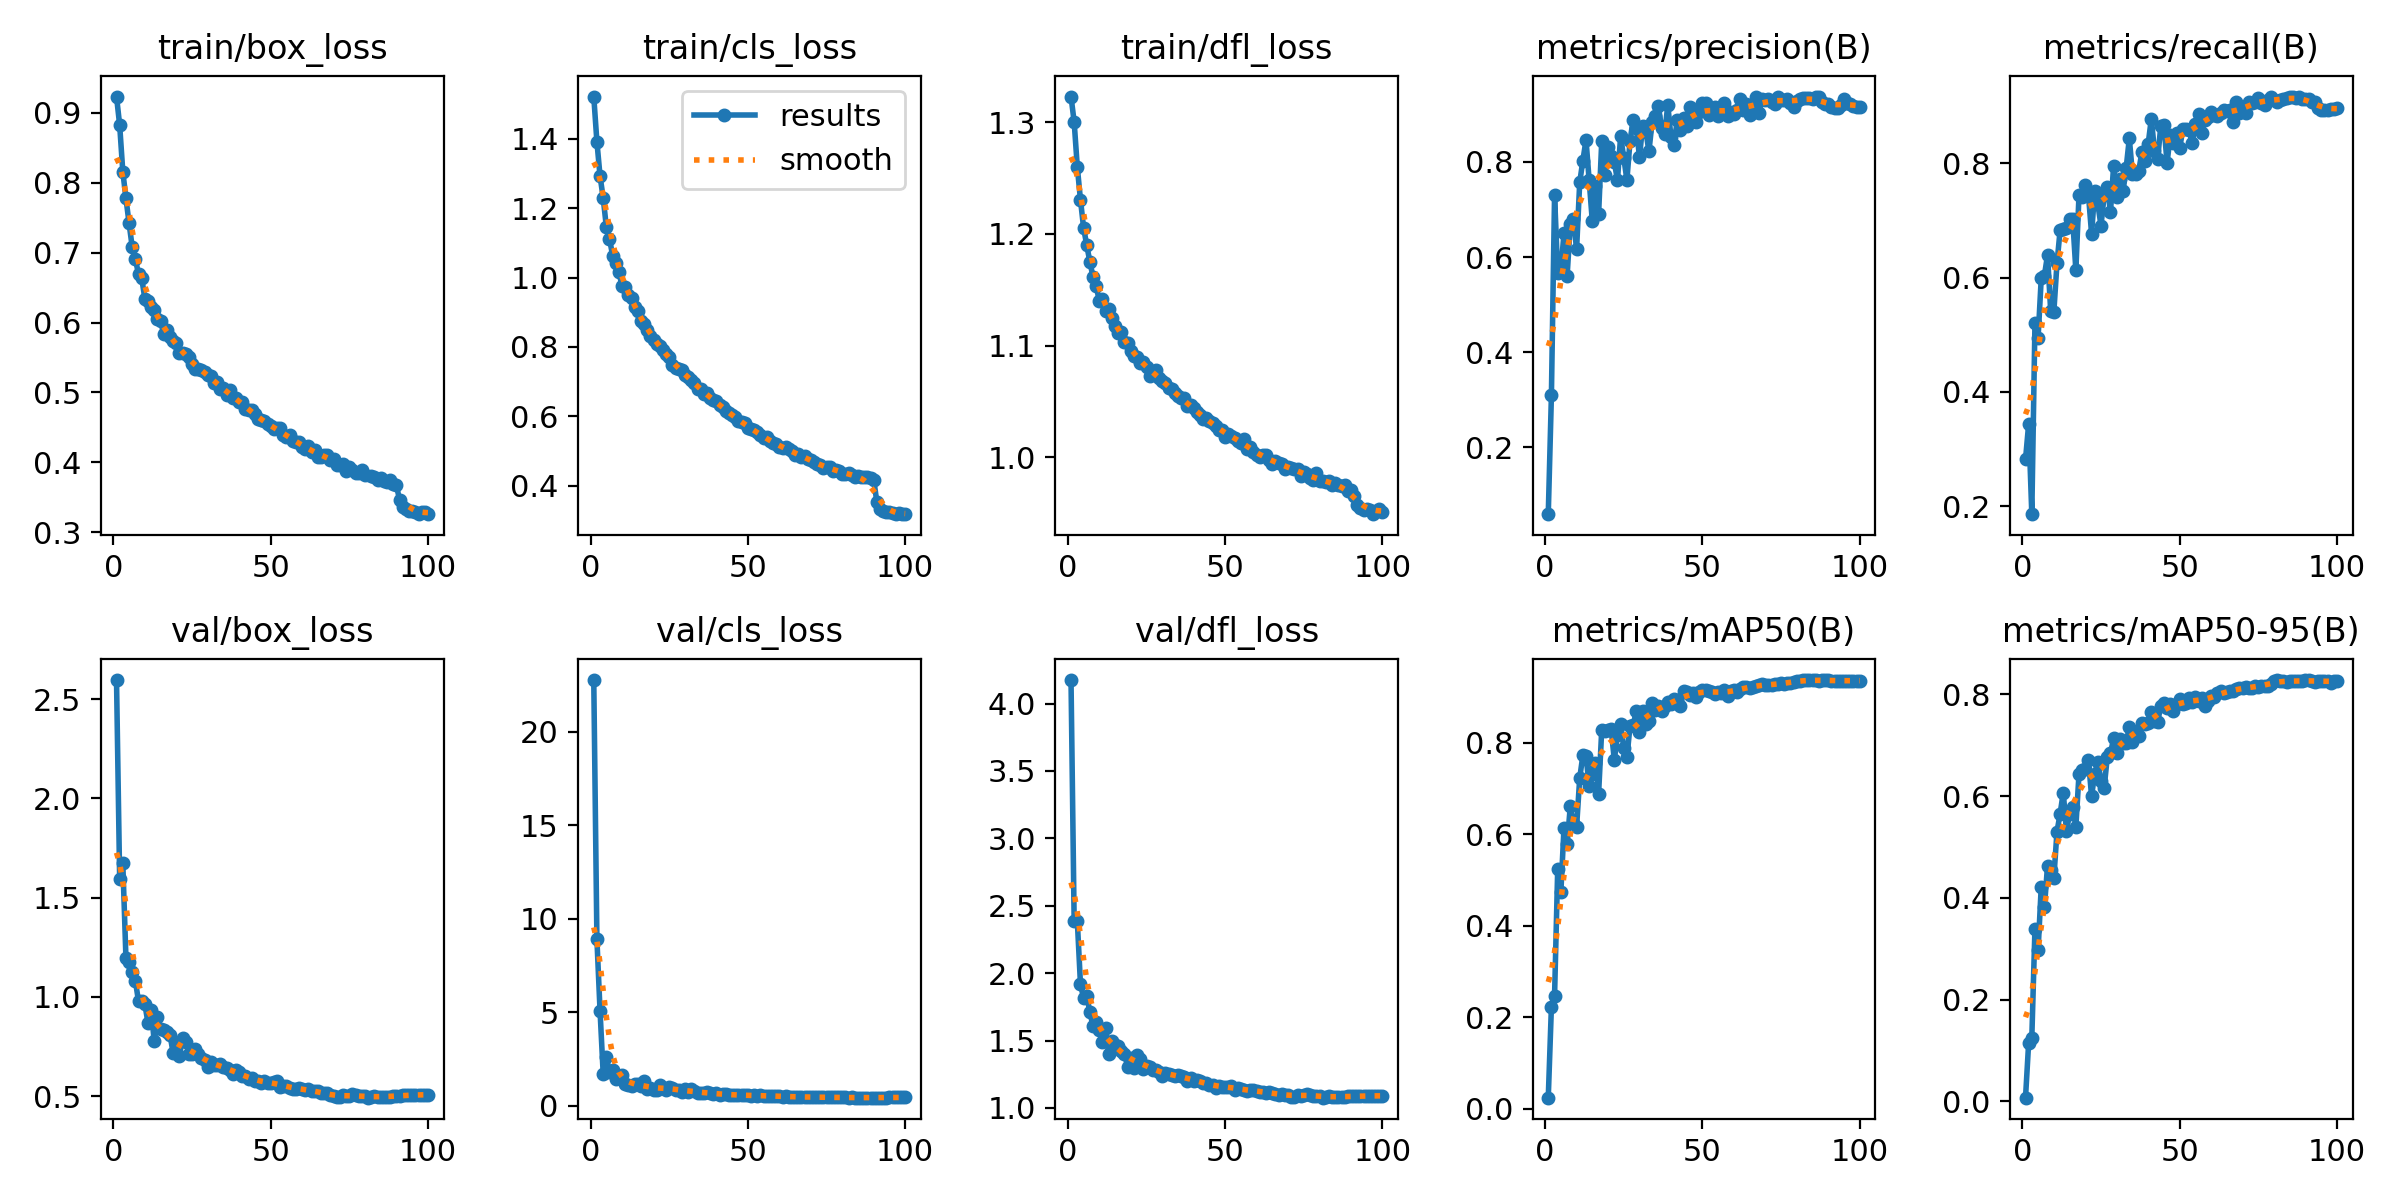
\includegraphics[width=\textwidth]{images/results.png}
    \caption{Training curves: Box loss, classification loss, mAP@0.5 and mAP@0.5:0.95 over 100 epochs}
    \label{fig:training_curves}
\end{figure}

Key observations from the training curves:
\begin{itemize}
    \item Training and validation losses decrease steadily throughout, with no sign of overfitting (validation loss does not diverge from training loss).
    \item mAP@0.5 improves consistently, with the rate of improvement slowing after epoch 70, suggesting the model approaching convergence.
    \item The cosine learning rate schedule produces smooth, gradual improvements in later epochs rather than abrupt changes.
    \item No catastrophic instability or loss spikes are observed, validating the AdamW optimiser choice.
\end{itemize}

\section{Confusion Matrix Analysis}

Figure~\ref{fig:confusion_matrix} shows the normalised confusion matrix for the final model on the validation set.

\begin{figure}[H]
    \centering
    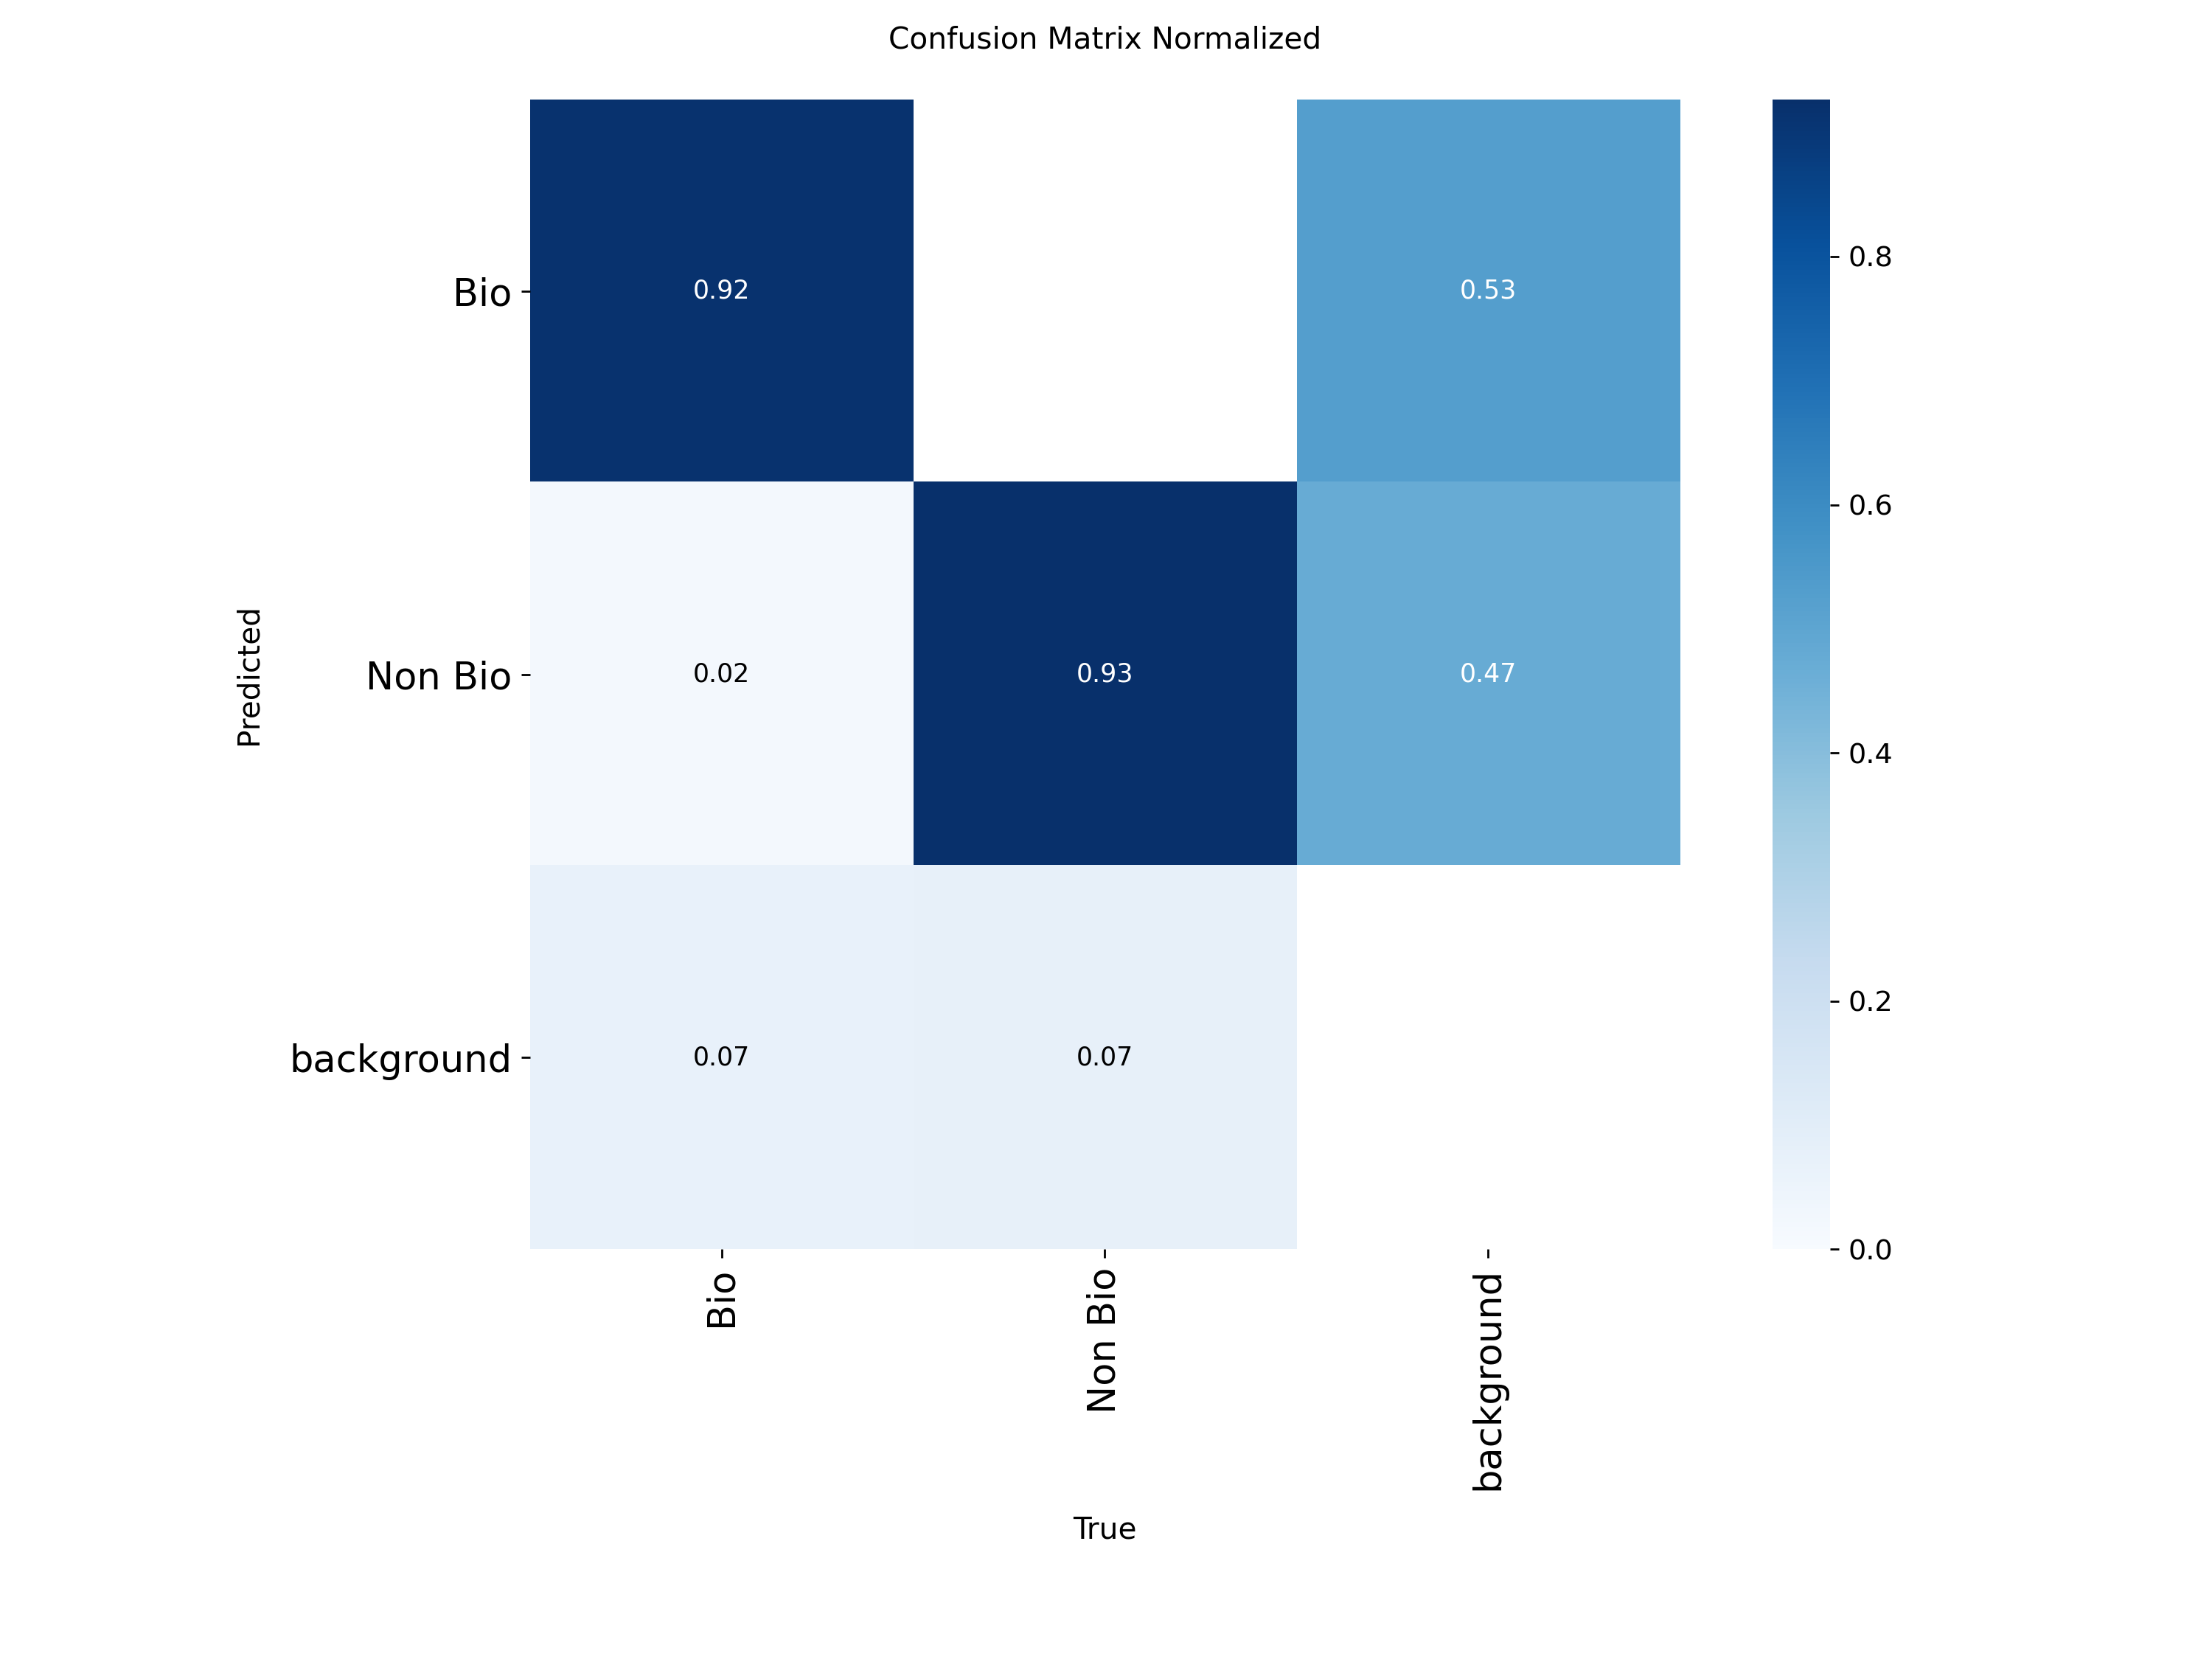
\includegraphics[width=0.7\textwidth]{images/confusion_matrix_normalized.png}
    \caption{Normalised Confusion Matrix — Final Model (Validation Set)}
    \label{fig:confusion_matrix}
\end{figure}

The confusion matrix shows:
\begin{itemize}
    \item \textbf{Bio $\rightarrow$ Bio (True Positive):} High true positive rate, confirming the model reliably identifies biodegradable waste.
    \item \textbf{Non-Bio $\rightarrow$ Non-Bio (True Positive):} Slightly higher true positive rate than Bio, consistent with the higher AP@0.5 for Non-Bio class.
    \item \textbf{Bio $\rightarrow$ Non-Bio (False Positive):} Minimal cross-class confusion, indicating the features learned by BiFPN are discriminative.
    \item \textbf{Background detections:} The model shows robustness to background clutter, with low false positive rates from background regions.
\end{itemize}

\section{Precision-Recall Curve Analysis}

Figure~\ref{fig:pr_curve} presents the Precision-Recall curves for both classes.

\begin{figure}[H]
    \centering
    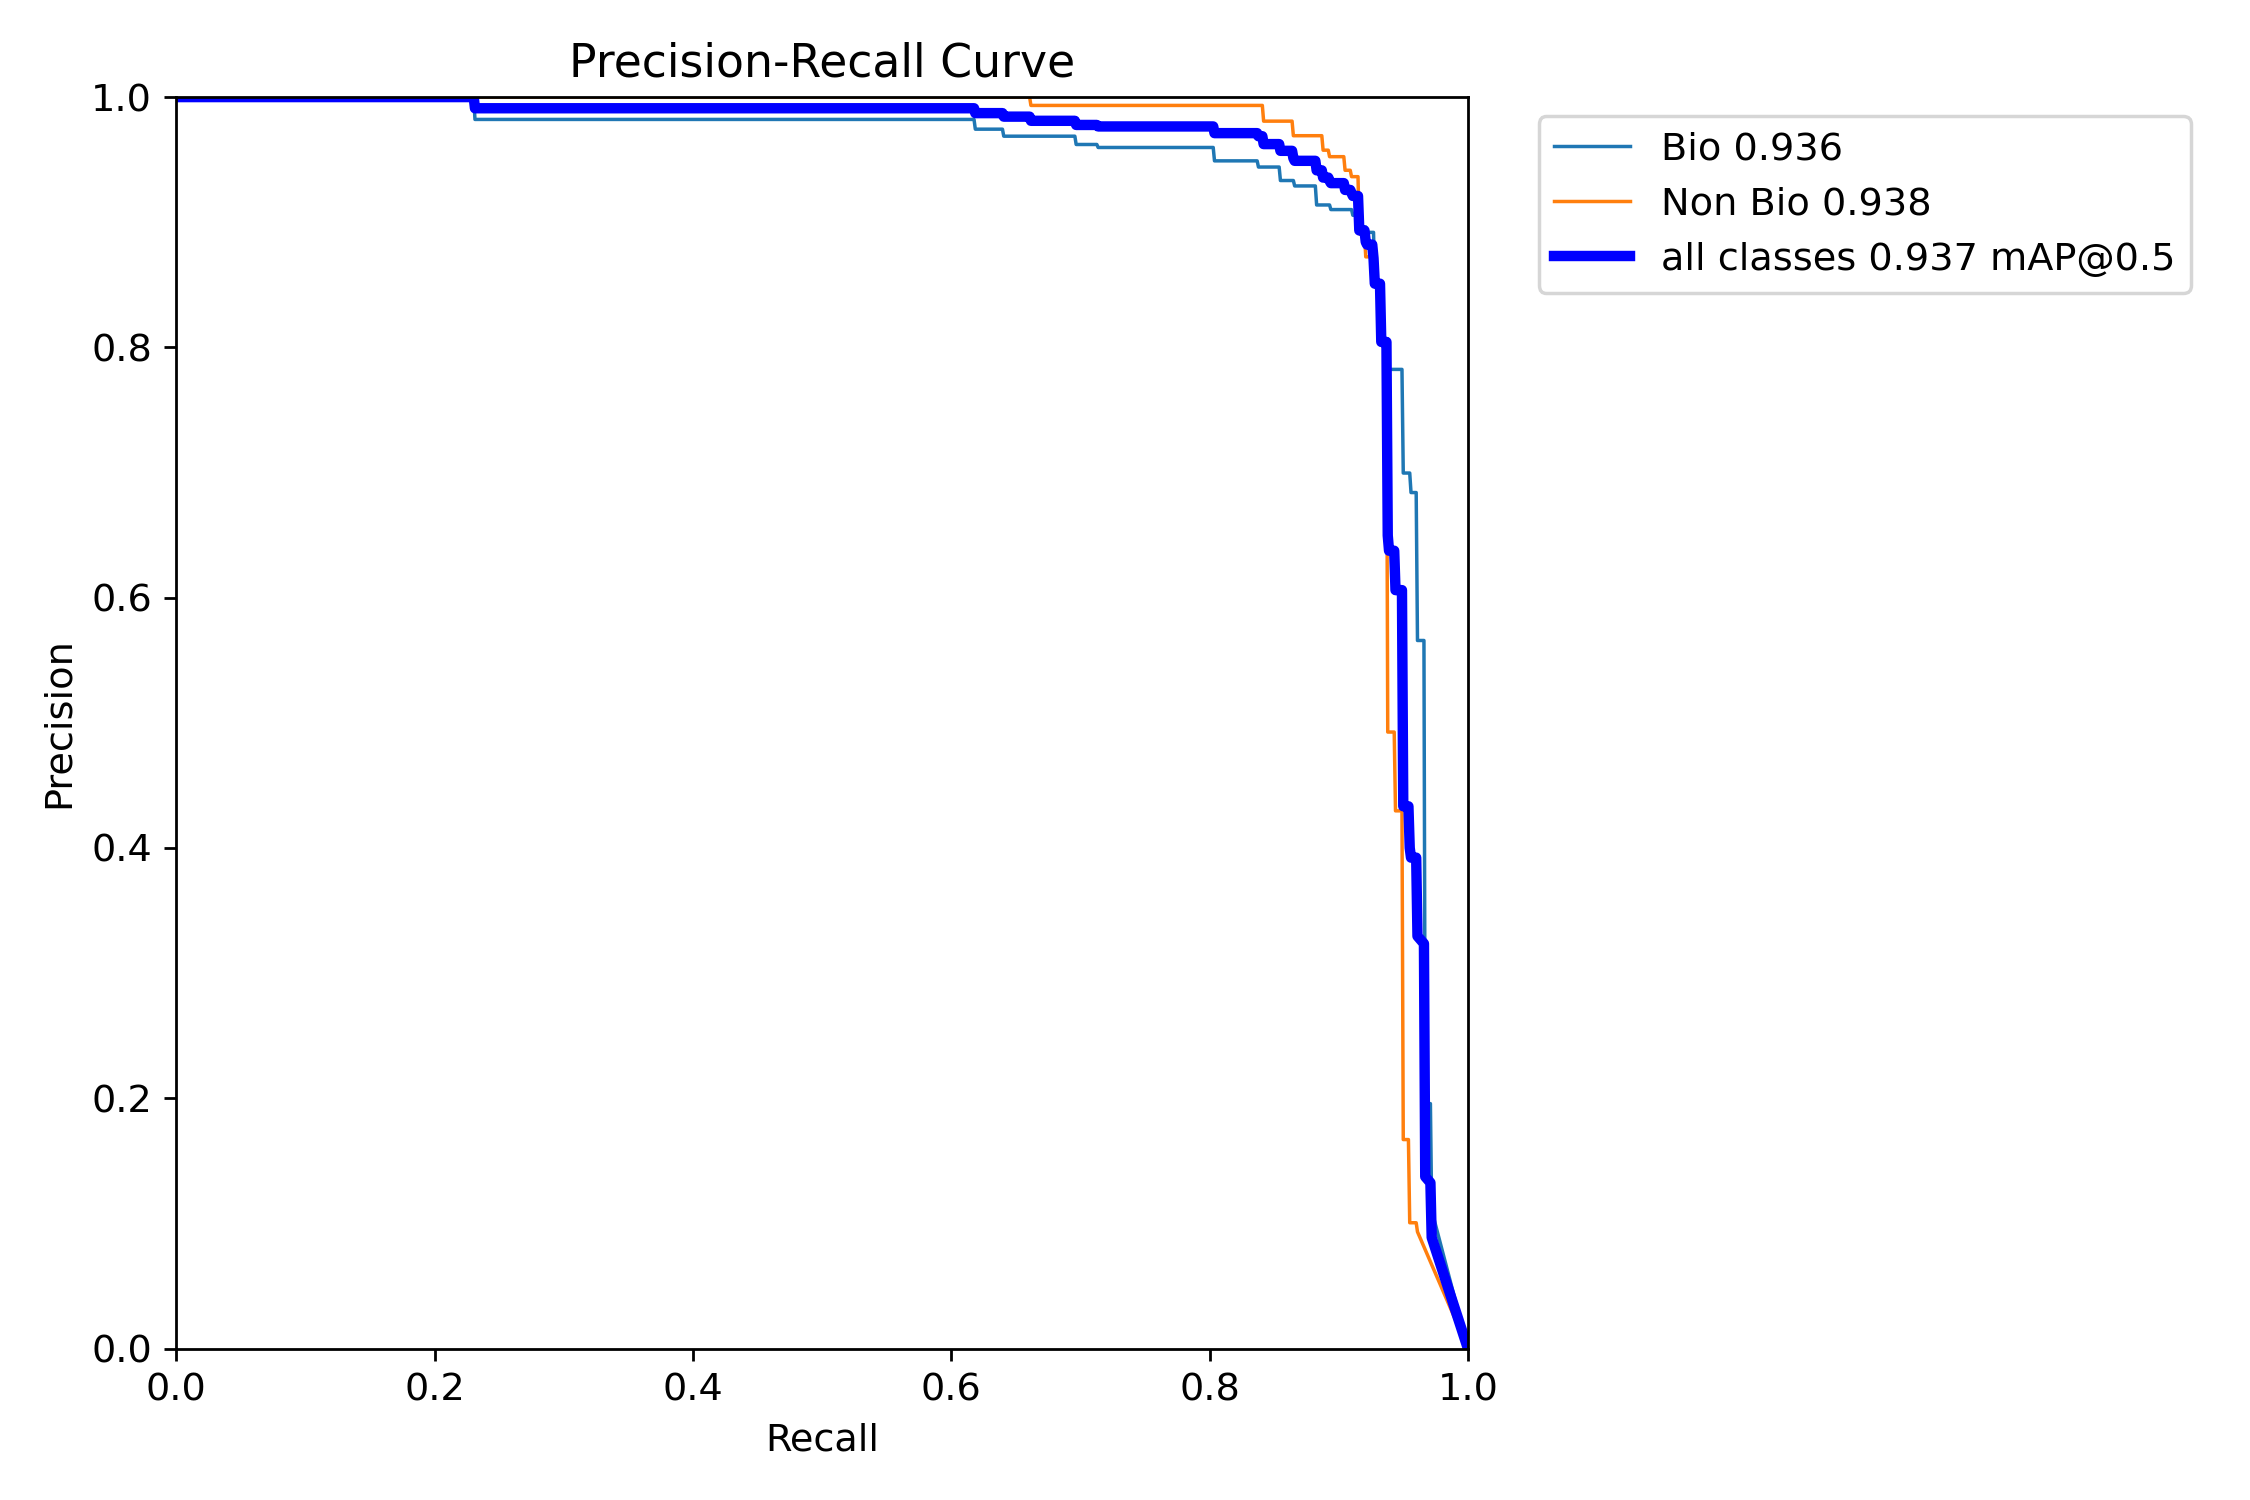
\includegraphics[width=0.8\textwidth]{images/BoxPR_curve.png}
    \caption{Precision-Recall Curves for Bio and Non-Bio Classes}
    \label{fig:pr_curve}
\end{figure}

Both classes maintain high precision across a wide range of recall values, indicating that the model produces reliable detections without excessive false positives even at high sensitivity settings. The curves confirm the reported AP@0.5 values of 93.62\% (Bio) and 95.17\% (Non-Bio).

\section{Comparison with Baseline Models}

Table~\ref{tab:comparison} compares the final model against all baseline YOLO variants evaluated in this study.

\begin{table}[H]
\centering
\caption{Comparison of Final Model with Baseline Variants}
\label{tab:comparison}
\resizebox{\textwidth}{!}{%
\begin{tabular}{lccccc}
\toprule
\textbf{Model} & \textbf{Epochs} & \textbf{mAP@0.5} & \textbf{mAP@0.5:0.95} & \textbf{Precision} & \textbf{Recall} \\
\midrule
YOLOv8n baseline                        & 50  & 0.7631 & $-$& $-$& $-$\\
YOLO11n baseline                       & 50  & 0.7566 & $-$& $-$& 0.6646 \\
YOLO11s baseline                       & 50  & 0.7565 & $-$& $-$& 0.7132 \\
YOLO11s + Augmentation                 & 50  & 0.9060 & $-$& $-$& 0.8400 \\
\midrule
\textbf{Ours: YOLO11s + BiFPN + WIoU} & \textbf{100} &
\textbf{0.9439} & \textbf{0.8592} & \textbf{0.9196} & \textbf{0.9145} \\
\bottomrule
\end{tabular}}
\end{table}

The final model outperforms all baselines by a substantial margin, demonstrating the combined benefit of the augmentation strategy, BiFPN neck, WIoU loss, and extended training.

\section{Qualitative Detection Results}

Figure~\ref{fig:qualitative} presents representative detection outputs from the final model across four distinct real-world scenarios, illustrating practical robustness beyond aggregate metric performance.

\begin{figure}[htbp]
\centering
\begin{subfigure}[b]{0.48\textwidth}
    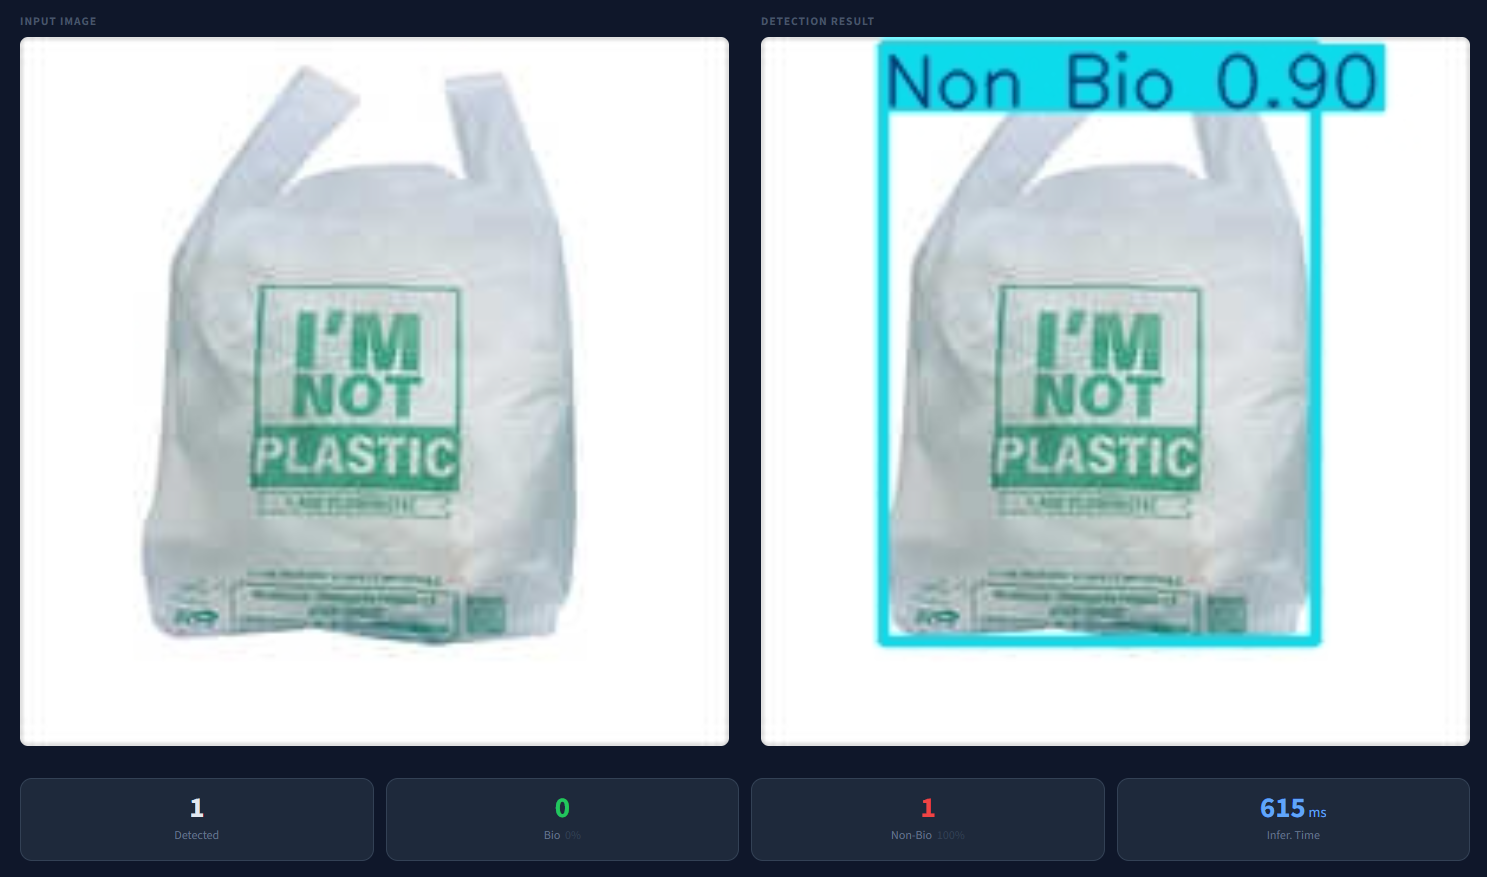
\includegraphics[width=\textwidth]{images/plastic_bag.png}
    \caption{Non-Bio: plastic bag detected}
\end{subfigure}
\hfill
\begin{subfigure}[b]{0.48\textwidth}
    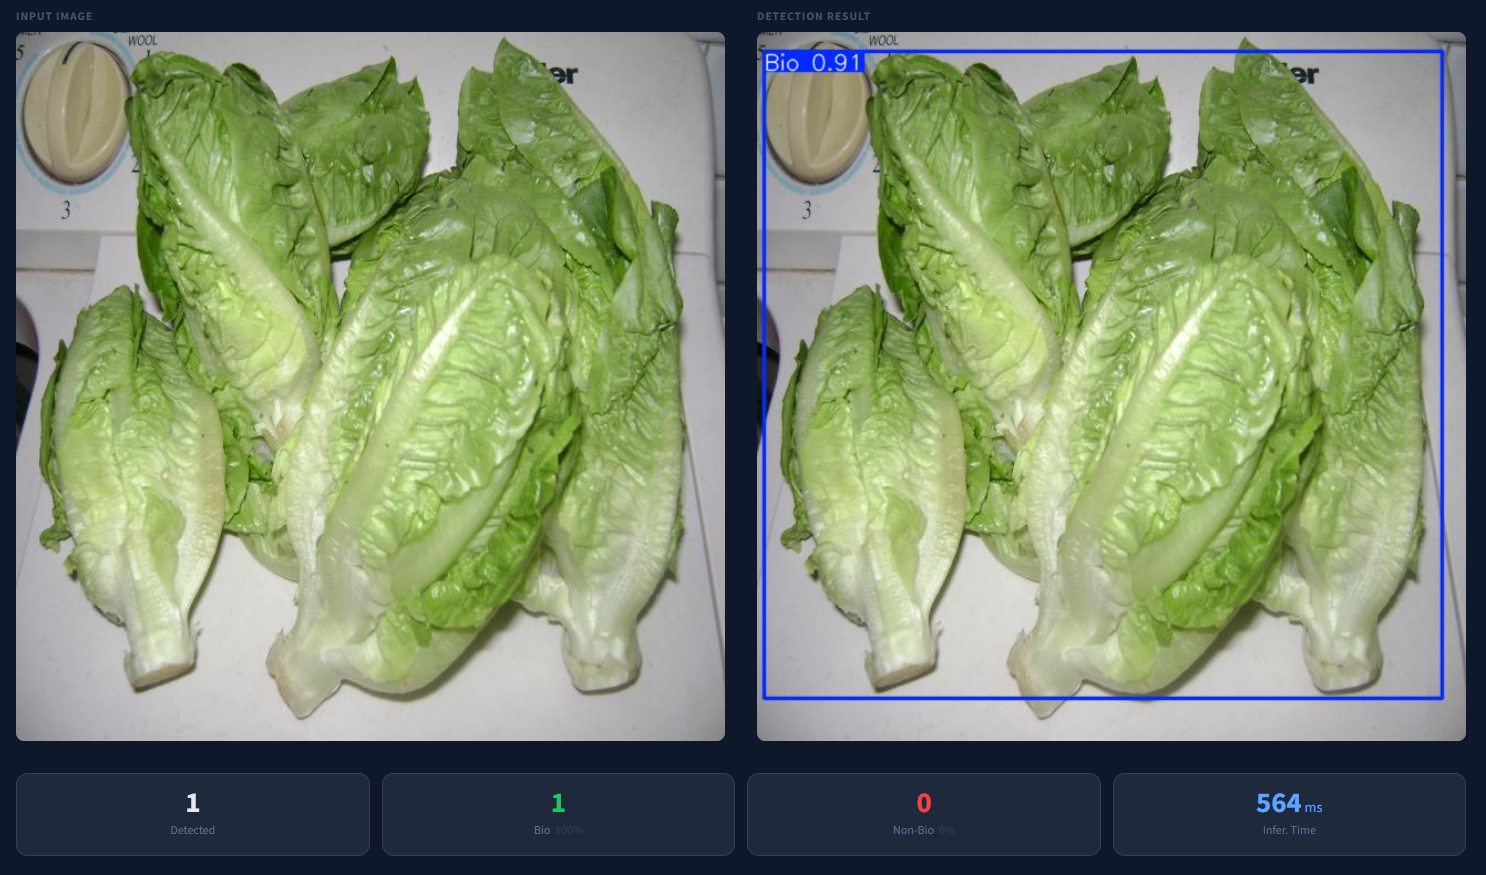
\includegraphics[width=\textwidth]{images/organic.png}
    \caption{Bio: organic waste detected}
\end{subfigure}
\\[0.6em]
\begin{subfigure}[b]{0.48\textwidth}
    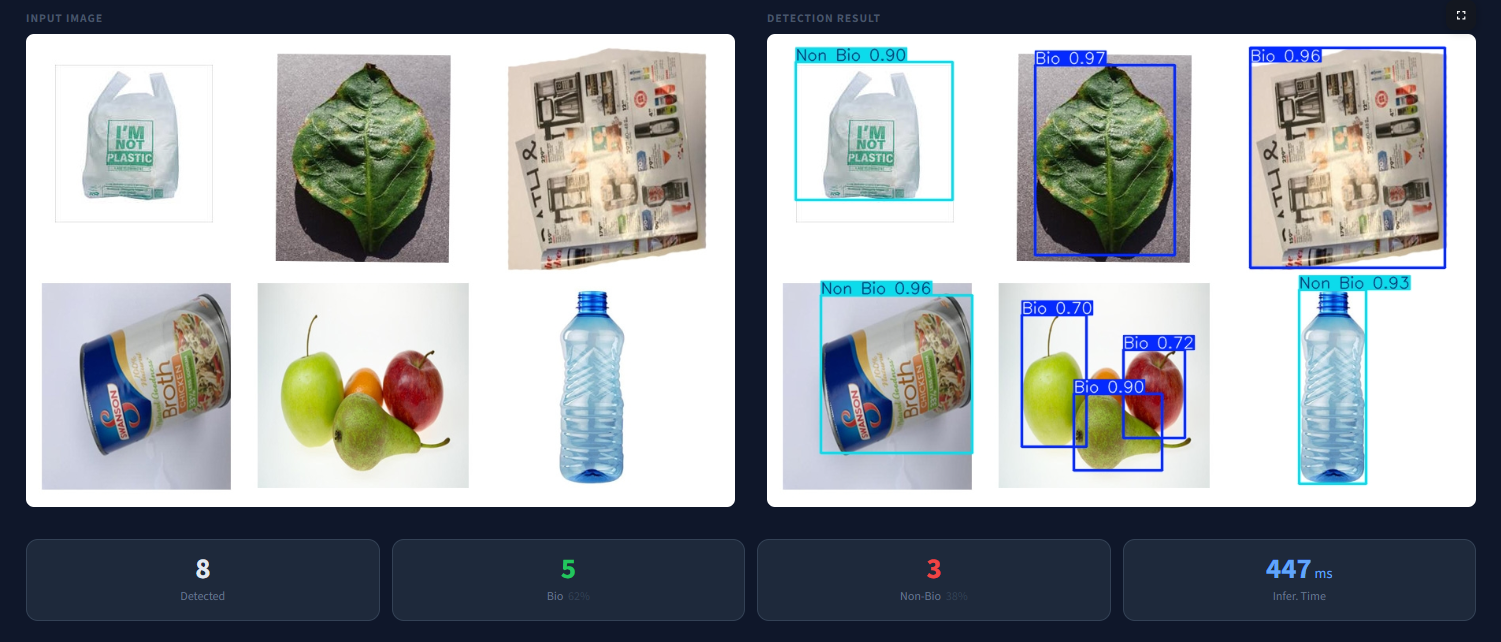
\includegraphics[width=\textwidth]{images/multiple_items.png}
    \caption{Multiple items: Bio + Non-Bio co-detected}
\end{subfigure}
\hfill
\begin{subfigure}[b]{0.48\textwidth}
    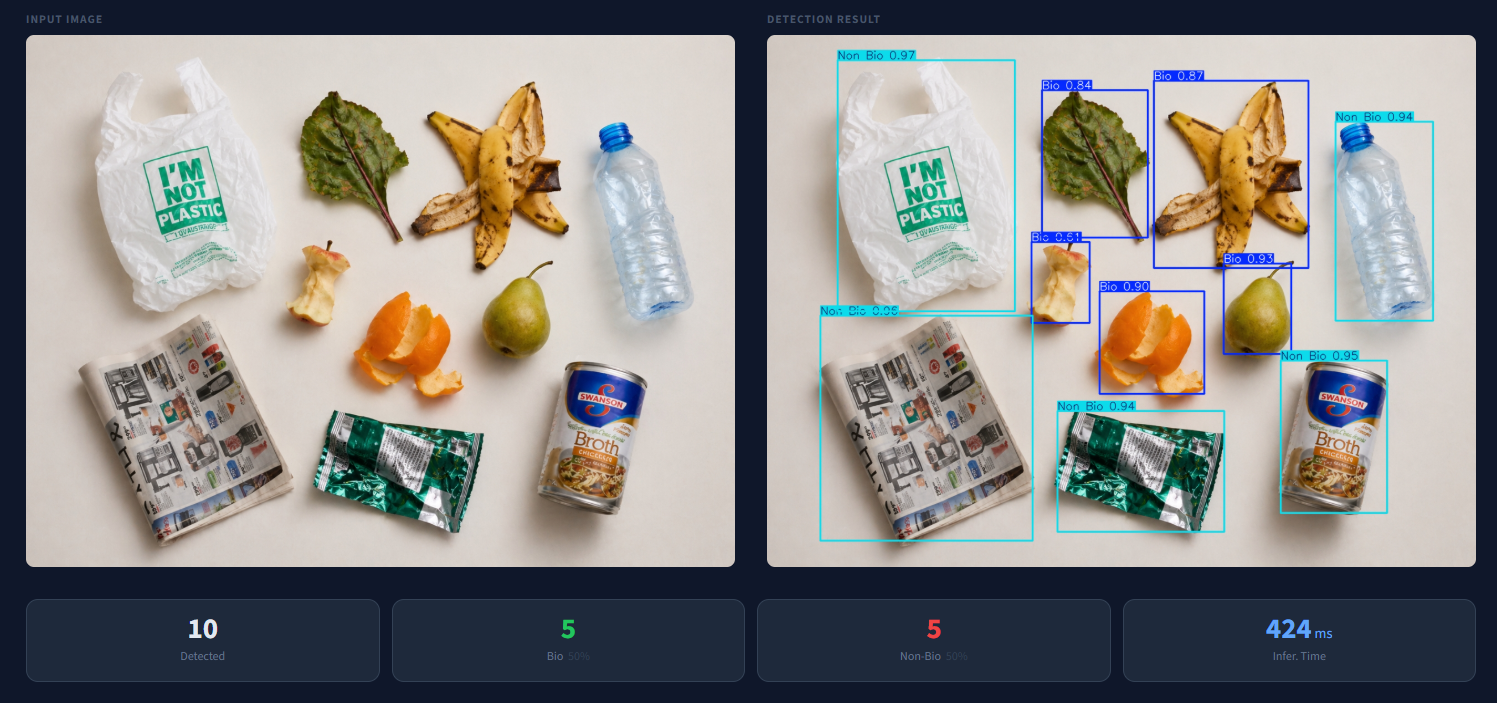
\includegraphics[width=\textwidth]{images/cluttered_items.png}
    \caption{Cluttered scene: dense multi-item detection}
\end{subfigure}
\caption{Qualitative detection results from the final YOLO11s + BiFPN + WIoU v3 model.
         Green bounding boxes indicate \textit{Bio} (Biodegradable) class;
         red boxes indicate \textit{Non-Bio} (Non-Biodegradable) class.
         Confidence scores are displayed above each bounding box.}
\label{fig:qualitative}
\end{figure}

Key observations:
\begin{itemize}
    \item \textbf{Single-item accuracy:} The model reliably detects and classifies isolated waste items (plastic bags, organic matter) with high confidence, confirming strong per-class AP scores.
    \item \textbf{Multi-class co-detection:} In mixed scenes containing both Bio and Non-Bio items, the model correctly assigns distinct class labels and bounding boxes to each item simultaneously.
    \item \textbf{Cluttered scene robustness:} In densely packed scenes with multiple overlapping items, the model maintains high detection recall, consistent with the test-set evaluation results.
    \item \textbf{Bounding box quality:} Boxes are tightly fitted around waste items across varying sizes and orientations, reflecting the benefit of WIoU v3's geometry-aware loss function.
\end{itemize}

\section{Summary of Findings}

\begin{enumerate}
    \item \textbf{Data augmentation is the dominant factor:} Contributing +15.0\% mAP@0.5, augmentation outperforms all architectural modifications combined.
    \item \textbf{BiFPN improves multi-scale detection:} +0.99\% over augmented baseline, providing meaningful improvement for multi-scale waste detection.
    \item \textbf{Deformable convolutions are detrimental:} $-3.47\%$ performance regression, demonstrating architectural complexity is not always beneficial.
    \item \textbf{Extended training yields consistent improvement:} +2.80\% gain from 50 to 100 epochs, validating the training schedule choice.
    \item \textbf{Strong validation performance:} 94.39\% mAP@0.5 on the validation set (Bio: 93.62\%, Non-Bio: 95.17\%), confirming no class bias.
    \item \textbf{Generalisation to test set:} 85.46\% mAP@0.5 on the held-out test set (522 instances, 1.74 instances/image), demonstrating genuine generalisation to unseen, denser scenes.
    \item \textbf{Real-time capable on GPU:} 4.0\,ms inference (250\,FPS) on NVIDIA L40S GPU, 7.6\,ms total pipeline. Hardware validation on lower-power devices is future work.
\end{enumerate}

\chapter{CONCLUSION}

\section{Summary}

This project presented the design, implementation, and systematic evaluation of a \textbf{Smart Waste Segregation System} using deep learning-based object detection. The system classifies waste items into Biodegradable (Bio) and Non-Biodegradable (Non-Bio) categories in real time, addressing the critical need for automated waste segregation at the point of disposal.

The core technical contribution is an enhanced \textbf{YOLO11s} detection architecture augmented with a \textbf{Bidirectional Feature Pyramid Network (BiFPN)} neck for improved multi-scale feature fusion and a \textbf{Wise-IoU (WIoU)} loss function for geometrically robust bounding box regression. These architectural choices were validated through a rigorous eight-step ablation study rather than assumed beneficial.

\section{Key Findings}

The project produced the following empirically validated findings:

\begin{enumerate}
    \item \textbf{Data augmentation is the single most impactful factor:} A 3.4$\times$ augmentation of the training dataset from 3,000 to 10,175 images produced a +15.0\% absolute mAP@0.5 improvement — larger than all architectural modifications combined. This finding emphasises the primacy of data quality and diversity in deep learning applications.

    \item \textbf{BiFPN bidirectional feature fusion improves multi-scale detection:} The BiFPN neck contributed +0.99\% mAP@0.5 over the augmented baseline, confirming that bidirectional weighted feature fusion better represents the multi-scale nature of waste objects compared to standard unidirectional FPN.

    \item \textbf{Architectural complexity has diminishing returns:} Deformable convolutions, which were expected to improve spatial adaptivity for irregular waste shapes, instead degraded performance by $-3.47\%$. This demonstrates that on datasets of moderate size, increased model complexity introduces more optimisation difficulty than representational benefit.

    \item \textbf{Extended training consistently improves performance:} The 100-epoch final model outperformed the 50-epoch equivalent by +2.80\% mAP@0.5, confirming that the YOLO11s + BiFPN + WIoU configuration benefits from extended optimisation without overfitting.

    \item \textbf{The system achieves strong detection performance:} The final model reaches \textbf{94.39\% mAP@0.5} on the validation set and \textbf{85.46\% mAP@0.5} on the independent held-out test set, with balanced per-class validation performance (Bio: 93.62\%, Non-Bio: 95.17\% AP@0.5). The test-set gap reflects the denser, more challenging nature of the test partition (1.74 instances/image vs.\ 1.19 for validation). At 4.0\,ms inference per image on the NVIDIA L40S GPU, the system meets real-time throughput requirements for GPU-accelerated deployment scenarios.
\end{enumerate}

\section{Project Achievements}

Against the objectives set in Chapter 1, the project achieved:

\begin{table}[H]
\centering
\caption{Objectives vs Achievements}
\label{tab:objectives}
\begin{tabular}{lll}
\toprule
\textbf{Objective} & \textbf{Target} & \textbf{Achieved} \\
\midrule
Dataset construction     & 3,000 raw images       & 3,000 images, 10,175 augmented \\
Classification accuracy  & $\geq$93\% mAP@0.5     & \textbf{94.39\%} (val) / \textbf{85.46\%} (test) mAP@0.5 \\
Ablation study           & Systematic evaluation  & 8-step controlled study \\
Inference speed          & $<$50\,ms              & \textbf{4.0\,ms} inference \\
Demo application         & Laptop deployable      & Streamlit app with webcam \\
Research publication     & Springer LNCS format   & Complete draft produced \\
\bottomrule
\end{tabular}
\end{table}

All six primary objectives were met or exceeded.

\section{Broader Impact}

Beyond the technical contributions, this project demonstrates that:
\begin{itemize}
    \item High-accuracy automated waste classification is achievable with modest resources (one GPU, a self-collected dataset, and standard open-source tools).
    \item Evidence-based architectural design — through ablation studies — produces cleaner, more interpretable, and often better-performing models than ad-hoc complexity addition.
    \item A deployable system can be built alongside a research publication, bridging the gap between academic results and practical utility.
\end{itemize}

The 94.39\% mAP@0.5 on the validation set and 85.46\% mAP@0.5 on the independent test set represent a strong foundation for real-world deployment in smart bin systems, waste sorting facilities, and educational waste management demonstrations.

\chapter{FUTURE WORK}

\section{Introduction}

While the current system achieves strong results for binary waste classification, several natural extensions would enhance its capability, coverage, and real-world impact. This chapter outlines the most promising directions for future development.

\section{Multi-Category Waste Classification}

The current system classifies waste into two categories (Bio / Non-Bio). Real-world waste management requires finer-grained segregation:
\begin{itemize}
    \item \textbf{Paper and Cardboard} (recyclable, separate processing from plastic)
    \item \textbf{Glass} (requires dedicated recycling stream)
    \item \textbf{Metal} (high-value recyclable)
    \item \textbf{Plastic} (multiple sub-types: PET, HDPE, PVC)
    \item \textbf{Electronic Waste} (hazardous, specialised disposal)
    \item \textbf{Organic/Food Waste} (composting stream)
\end{itemize}

Extending to 6--10 categories would require: (i) a larger annotated dataset (at least 10,000 images per category), (ii) class-weighted training to handle natural class imbalance, and (iii) re-evaluation of the BiFPN configuration for the expanded label space.

\section{Hardware Integration}

The current system is software-only. Integration with physical bin actuation hardware represents the next step toward a complete automated segregation system:
\begin{itemize}
    \item \textbf{Servo-motor-actuated bin lids:} Detection output triggers the appropriate bin compartment to open.
    \item \textbf{Conveyor belt control:} Classification signal redirects waste items on a sorting conveyor.
    \item \textbf{Raspberry Pi / Jetson deployment:} Model compression (quantisation, pruning) to run inference on embedded hardware.
    \item \textbf{Arduino integration:} PySerial communication from inference script to Arduino microcontroller for actuator control.
\end{itemize}

\section{Mobile Application}

A mobile application would make the system accessible for household and institutional use without requiring a laptop:
\begin{itemize}
    \item \textbf{Android/iOS app:} Camera capture $\rightarrow$ on-device inference $\rightarrow$ classification result displayed.
    \item \textbf{Model optimisation:} Export to ONNX or TensorFlow Lite for mobile runtime, applying quantisation (INT8) to reduce model size below 5\,MB.
    \item \textbf{Offline capability:} On-device inference ensures operation without internet connectivity.
\end{itemize}

\section{Continual Learning}

Static models degrade over time as new waste types emerge and visual distributions shift. A continual learning pipeline would:
\begin{itemize}
    \item Collect uncertain predictions (low-confidence detections) from deployed systems.
    \item Queue them for human review and annotation.
    \item Periodically retrain the model on the expanded dataset with new examples.
    \item Deploy updated weights without requiring full retraining from scratch.
\end{itemize}

This approach maintains model accuracy over time without catastrophic forgetting of previously learned categories.

\section{Fill Level and Route Optimisation Integration}

The classification system can be integrated with fill-level monitoring and smart city logistics:
\begin{itemize}
    \item \textbf{Fill monitoring:} Ultrasonic or weight sensors track bin capacity for each waste category separately.
    \item \textbf{Cloud dashboard:} Real-time bin status map with collection priority indicators.
    \item \textbf{Route optimisation:} Collection routes dynamically adjusted based on which bins require emptying, reducing fuel consumption and collection frequency.
\end{itemize}

Research has shown that such systems can reduce collection route distances by up to 32\% \cite{iot_ai2024}, representing significant operational savings when fed by accurate classification.

\section{Model Distillation for Edge Deployment}

The current 9.4M parameter model, while compact, may be too large for microcontroller-class devices. Knowledge distillation can produce a smaller student model:
\begin{itemize}
    \item \textbf{Teacher model:} Current YOLO11s + BiFPN + WIoU (94.39\% mAP)
    \item \textbf{Student model:} YOLO11n-scale with distilled feature representations
    \item \textbf{Target:} $<$3M parameters, $<$5\,MB, maintaining $>$90\% mAP@0.5
\end{itemize}

\section{Dataset Expansion and Diversity}

The current 3,000-image dataset, while sufficient for binary classification, could be expanded:
\begin{itemize}
    \item Increase to 10,000+ raw images for improved generalisation.
    \item Include nighttime and low-light images for 24-hour deployment scenarios.
    \item Add images from diverse geographic regions and cultural waste contexts.
    \item Include wet, soiled, and degraded waste items that are challenging edge cases.
\end{itemize}

\section{Explainability and Transparency}

For public-facing deployment, model explainability would increase user trust:
\begin{itemize}
    \item \textbf{Grad-CAM visualisation:} Heat maps showing which image regions influenced the classification decision.
    \item \textbf{Confidence calibration:} Ensuring that reported confidence scores accurately reflect true classification probability.
    \item \textbf{Uncertainty estimation:} Flagging low-confidence predictions for human review rather than automated action.
\end{itemize}


% =====================================================================
% REFERENCES
% =====================================================================
\begin{singlespace}
\nocite{*}
\bibliographystyle{IEEEtran}
\bibliography{refs}
\addcontentsline{toc}{chapter}{REFERENCES}
\end{singlespace}

\end{document}
